\documentclass[11pt,a4paper]{article}

\usepackage[utf8]{inputenc}
\usepackage[T1]{fontenc}
\usepackage{geometry}
\geometry{a4paper, margin=2.5cm}
\usepackage{amsmath, amssymb, amsthm}
\usepackage{graphicx}
\usepackage{hyperref}
\usepackage{cite}
\usepackage{color}
\usepackage{braket} % For Dirac notation
\usepackage{mathrsfs} % For mathscr
\usepackage{dsfont} % For identity operator
\usepackage{lmodern} % Better font rendering

% Theorem environments
\newtheorem{theorem}{Theorem}[section]
\newtheorem{lemma}[theorem]{Lemma}
\newtheorem{proposition}[theorem]{Proposition}
\newtheorem{corollary}[theorem]{Corollary}
\newtheorem{definition}[theorem]{Definition}
\newtheorem{axiom}[theorem]{Axiom}
\newtheorem{postulate}[theorem]{Postulate}

% Custom commands
\newcommand{\ketomega}{|\Omega\rangle}
\newcommand{\hilbert}{\mathcal{H}}
\newcommand{\iu}{\mathrm{i}} % imaginary unit
\newcommand{\e}{\mathrm{e}} % Euler's number

\title{Omega Theory: Axiomatic Foundations of Holographic Spacetime and Interactive Evolution}
\author{Haobo Ma\thanks{Email: auric@aelf.io} \\
\textit{AELF PTE LTD.} \\
\textit{\#14-02, Marina Bay Financial Centre Tower 1, 8 Marina Blvd, Singapore 018981}}
\date{\today}

\begin{document}

\maketitle

\begin{abstract}
We propose and systematize a unified cosmological framework---Omega Theory---starting from the geometry of Hilbert space and a finite-information postulate. Based on the ``Omega Axiom,'' the physical universe is identified with a single, static, normalized vector $|\Omega\rangle$ in an infinite-dimensional separable Hilbert space; apparent dynamics arise from spectral decompositions and basis-dependent phase structure. Motivated by the Bekenstein--Hawking bound and the Holographic Principle, we introduce ``Finite Information'' and ``Holographic Mapping'' axioms that model finite causal regions by effective finite-dimensional Hilbert spaces encoded on lower-dimensional boundaries.

Building on this, we introduce a Quantum Cellular Automaton (QCA) on a quasicrystal background and analyze conditions under which a Dirac-like continuum limit and emergent relativistic symmetry obtain. By introducing a ``Golden Unitary'' ansatz driven by a Golden Ratio spectrum, we construct an evolution that is non-periodic in the projective Hilbert space and discuss its geometric visualization.

At the dynamical level, we define an Omega Action containing Fisher-information terms and derive the associated field equations in a minimal setting, outlining implications for cosmology and phenomenology (varying constants, high-energy dispersion, and holographic-noise templates). We further interpret gravitational time dilation as a computational routing overhead: the exact 1D nearest-neighbor compilation depth required to realize a local PQCA step defines an emergent lapse field. At the computational-ontological level, we treat the universe as an Interactive Quantum Automaton and propose an ``Observer Operator'' as a formal mechanism for discussing computability/incompleteness constraints and measurement-like selection. Supporting derivations and technical details are collected in the Appendices, including the quasicrystal continuum-limit analysis, the tensor-network holographic construction, and proposed geometric ans\"atze for internal symmetry and constants.
\end{abstract}

\textbf{Keywords}: Quantum Gravity, Holographic Principle, Quantum Cellular Automata, Foundations of Quantum Mechanics, Cosmology, Fine Structure Constant, Gödel Incompleteness.

\tableofcontents
\newpage

\part{Introduction and Context}
\label{part:I}

\section{Introduction and Motivation}
\label{chap:intro}

\subsection{The Tension in Fundamental Physics: Time and Information}
The early 21st century finds fundamental physics in a state of productive tension. The partial unification achieved in the 1970s has bifurcated into two mutually incompatible frameworks: Quantum Mechanics (QM), describing the micro-world as probabilistic, unitary, and time-reversible; and General Relativity (GR), describing the macro-world as deterministic, geometrical, and background-independent. The interface between them---quantum gravity---remains elusive, primarily due to the "Problem of Time."
In GR, time is a dynamical coordinate found by solving the field equations (diffeomorphism invariance). In QM, time is a background parameter driving unitary evolution. The Wheeler-DeWitt equation $\hat{H}|\Psi\rangle = 0$, the naive quantization of GR, implies a "frozen formalism" where the physical state of a closed universe does not evolve.

Furthermore, the discovery of black hole thermodynamics and the holographic principle \cite{bekenstein1973black,hawking1975particle,susskind1995world} provides a sharp constraint/motivation: the information content of any finite spatial region is bounded by its surface area, not its volume. This suggests that the continuous manifolds of GR and the local fields of QFT may be redundant descriptions of a more fundamental, lower-dimensional organization of degrees of freedom.

This paper proposes a unified framework---\textbf{Omega Theory}---which addresses the time problem by accepting the static nature of the quantum universe (The Omega Axiom) and reinterpreting change as an intrinsic, operationally accessible structure on the state (projective geometry / information processing). This viewpoint is compatible with relational and thermal-time perspectives on ``evolution without external time'' \cite{PageWootters1983,ConnesRovelli1994}. We model the microscopic substrate as a discrete, finite-informational structure (a Quantum Cellular Automaton) together with a holographic encoding architecture for emergent effective spacetime descriptions.

\begin{figure}[h]
    \centering
    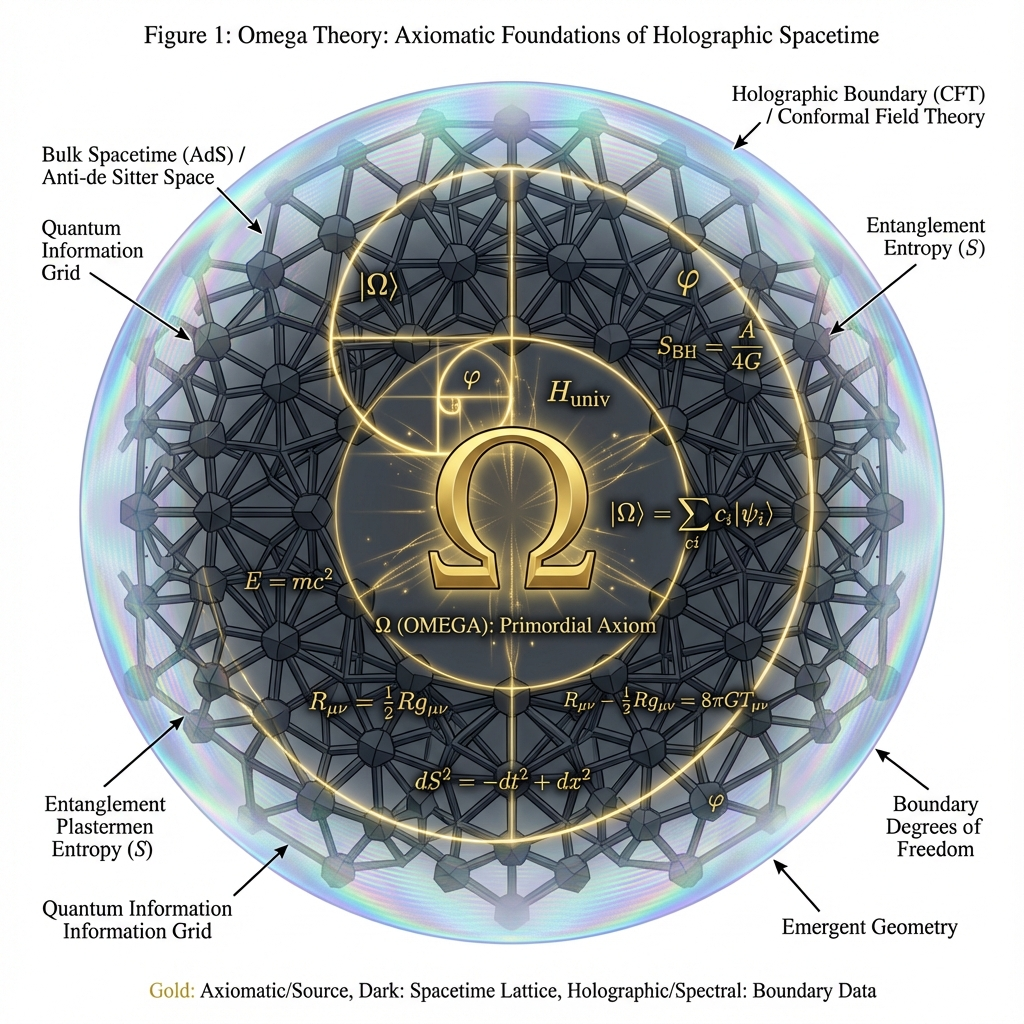
\includegraphics[width=0.8\textwidth]{images/omega_theory.png}
    \caption{Conceptual overview of Omega Theory: The static global vector $|\Omega\rangle$ yields an effective 4D spacetime description through holographic projection and quasicrystalline spectral/modular structure.}
    \label{fig:omega_concept}
\end{figure}

\subsection{Structure of the Argument}
Our argument proceeds in three layers, intended to separate rigorous foundations from specific models:
\begin{itemize}
    \item \textbf{Part I \& II (Foundations)}: We state the axioms around a global universe state $|\Omega\rangle$ and define intrinsic time via the geometry of projective Hilbert space (Fubini-Study metric). The finite-information/holographic input is treated as a working postulate that motivates an effectively discrete, local description.
    \item \textbf{Part III \& IV (Micro-Ontology)}: We propose a Quantum Cellular Automaton (QCA) on a quasicrystal network and analyze its Dirac continuum limit under explicit regularity assumptions. We then sketch how internal algebraic structure (octonions/$G_2$) could organize Standard Model-like quantum numbers, and we propose geometric ans\"atze for certain dimensionless constants.
    \item \textbf{Part V--VIII (Cosmology \& Interpretation)}: We introduce an information-geometric action principle (the Omega Action) and derive the associated field equations in a minimal setting. We outline cosmological/phenomenological consequences and discuss interpretational issues, including the role of observation in computationally incomplete dynamics.
\end{itemize}
For orientation, a compact dependency map of the main axioms, model assumptions, and derived templates is recorded in Appendix~\ref{sec:dependency_map}.

\section{Related Work and Positioning}
\label{chap:related_work}

Omega Theory does not exist in a vacuum. It synthesizes insights from several modern approaches but diverges in key ontological commitments.

\subsection{Relation to String Theory and AdS/CFT}
Like String Theory, we accept the Holographic Principle as central. However, unlike String Theory, which typically posits a background continuum (or an ensemble/landscape of vacua) and relies on string-scale excitations, Omega Theory is non-perturbative and background-independent from the start. Rather than invoking a landscape of distinct vacua, we postulate a single global state $\omega_\Omega$ (Axiom~O1); model-dependent ``vacuum data'' are encoded in the choice of that state and in the spectral/modular data of its restrictions to observer algebras.

\subsection{Relation to Loop Quantum Gravity (LQG)}
We share LQG's commitment to background independence and the discreteness of geometry (e.g.\ discrete spectra of kinematical area/volume operators) \cite{RovelliSmolin1995,AshtekarLewandowski1997Area}. However, deriving a fully controlled semiclassical limit together with a realistic low-energy matter sector remains challenging in current formulations; see, e.g., \cite{Perez2013SpinFoam,Thiemann2007}. Omega Theory sidesteps the direct quantization program by adopting a quantum-information substrate (a QCA) and treating both effective geometry and matter content as emergent in an appropriate coarse-grained limit.

\subsection{Relation to Causal Set Theory and Wolfram's Physics Project}
We share the vision that the universe is fundamentally a discrete graph or rewriting system (Causal Sets, Hypergraphs). However, most graph-based approaches struggle to recover quantum unitarity (the "Quantumness" problem). Omega Theory is strictly quantum-mechanical; the graph is treated as the tensor interaction structure of the Hilbert space, so microscopic unitarity is manifest in the regulated description.

\subsection{The Unique Contribution: Geometric Constants}
What sets Omega Theory apart is its attempt to relate dimensionless constants ($\alpha, \mu, \dots$) to geometric/topological data of the underlying informational construction, rather than treating them as arbitrary inputs. In this manuscript, these appear as explicit geometric ans\"atze; a full derivation from a unique microscopic measure and an explicit matching/RG closure remains an open task (Appendix~\ref{app:constants_proof}; Conjecture~\ref{conj:eft_matching}).

\subsection{Relation to Holographic Space-Time (HST) and Operator Algebras}
Omega Theory shares significant conceptual DNA with the \textbf{Holographic Space-Time (HST)} program of \textbf{Banks and Fischler} \cite{Banks2018}. Both approaches posit that spacetime is not fundamental but emerges from a finite quantum information structure, where the Hilbert space dimension determines the causal horizon area ($N \sim A/4G$). However, while HST constructs local causal diamonds dynamically, Omega Theory assumes a global static state $|\Omega\rangle$ from which causal diamonds are carved via tensor network disentanglers.

Furthermore, our identification of geometry with entanglement corresponds to the \textbf{Operator Algebra Quantum Error Correction (OAQEC)} framework \cite{Harlow2017, Pastawski2015}. The ``Golden MERA'' (Assumption~\ref{assump:M3}) is used here as a concrete tensor-network ansatz for the holographic encoding map postulated in Axiom~O4 \cite{Vidal2007MERA,Swingle2012MERA}, in the spirit of the HaPPY holographic pentagon code. The golden-spectrum update rule is an additional model assumption that supplies a specific intrinsic phase structure and a checkable dynamics/diagnostics layer for the ansatz, rather than a uniquely derived consequence of holography.

\section{Scope, Results, and Assumptions}
\label{chap:scope}

To facilitate verification, we state explicitly which elements are postulated, which are derived within the model, and which remain programmatic.

\subsection{Postulates (Axioms)}
\begin{itemize}
    \item \textbf{O1 (Omega Axiom)}: The universe is specified by a unique normalized global state $\omega_\Omega$ on a quasi-local operator algebra associated with a countable graph of finite-dimensional local degrees of freedom; there is no external time parameter \cite{BratteliRobinson1987OAQSM1}.
    \item \textbf{O2 (Finite Information)}: For any causally closed region with boundary area $A$, the effective dimension obeys $\dim \mathcal{H}_{\mathrm{region}} \le \exp(A/4l_P^2)$ \cite{bekenstein1973black,hawking1975particle,thooft1993dimensional,susskind1995world,Bousso2002}.
    \item \textbf{O3 (Causal Locality)}: There exists a discrete-time unitary update $\hat{U}$ with finite-range causal propagation: local observables evolve to observables supported only on bounded neighborhoods \cite{Watrous1995QCA,SchumacherWerner2004,Dariano2014}.
    \item \textbf{O4 (Holographic Mapping)}: There exists a holographic encoding map $\Phi$ from bulk to boundary which is an approximate isometry on the relevant code subspace and supports approximate OAQEC/entanglement-wedge reconstruction \cite{AlmheiriDongHarlow2015,Pastawski2015,Harlow2017}.
    \item \textbf{O5 (Scan--projection readout)}: Operational time and outcome statistics are obtained from finite-resolution scan and projection of intrinsic phase data (with standard consequences such as Sturmian readouts and canonical Ostrowski/Zeckendorf tick coordinates recorded as propositions in Part~II and Appendix) \cite{MorseHedlund1940,Lothaire2002,Zeckendorf1972,AlloucheShallit2003,Ma2025HPA}.
    \item \textbf{O6 (Unitary scan algebra)}: The scan is implemented by a nontrivial unitary $U_{\mathrm{scan}}$ with a conjugate unitary $V$ forming a Weyl pair, encoding intrinsic noncommutativity and uncertainty tradeoffs \cite{Weyl1916,Rieffel1981IrrationalRotations}.
\end{itemize}

\subsection{Model assumptions (concrete realization)}
\begin{itemize}
    \item \textbf{M1 (Icosahedral/quasicrystalline isotropy)}: The underlying graph is realized as an icosahedral quasicrystal ensuring statistical isotropy in the continuum limit (Assumption~\ref{assump:M1}).
    \item \textbf{M2 (Internal fiber and $G_2$ structure)}: Each site carries an $8$-dimensional internal sector organized by octonionic/$G_2$ structure (Assumption~\ref{assump:M2}).
    \item \textbf{M3 (Golden MERA / golden-spectrum update)}: A specific Golden MERA implementation of $\Phi$ and a golden-spectrum local update rule are adopted (Assumption~\ref{assump:M3}).
\end{itemize}

\subsection{Auxiliary assumptions}
\begin{itemize}
    \item \textbf{S1 (Readout-kernel symmetry)}: Microstate-counting normalizations assume a symmetric sharp-readout limit of the induced readout kernel (Assumption~\ref{assump:S1}).
    \item \textbf{C1 (Cosmological near-saturation)}: Cosmological scaling relations assume near-saturation of the holographic bound on horizon scales (Assumption~\ref{assump:C1}).
\end{itemize}

\subsection{Results derived in this manuscript (given the postulates)}
\begin{itemize}
    \item \textbf{Geometric time}: Intrinsic duration is identified with Fubini--Study distance in projective Hilbert space (Part II).
    \item \textbf{Omega Action variation}: A minimal information-geometric action yields modified Einstein equations with an ``information'' stress tensor, by direct variational calculus (Part V; Appendix \ref{app:action_proof}).
    \item \textbf{Dirac continuum limit (baseline and conditional extension)}: For the translation-invariant 1D coined walk, the long-wavelength limit yields Dirac evolution with a controlled lattice error (Part~III; Appendix~\ref{app:homogenization}). For quasicrystal/Fibonacci textures we provide explicit diagnostics on periodic approximants and quantify sensitivity to phason strain (Part~III; Appendix~\ref{app:fib_dqca}). The higher-dimensional homogenization target is isolated in Conjecture~\ref{conj:quasicrystal_dirac} and reduced to two quantitative control tasks in Appendix~\ref{app:homogenization}, Proposition~\ref{prop:quasicrystal_homogenization_reduction}.
\end{itemize}

\subsection{Programmatic components and open problems}
We isolate the remaining programmatic tasks into checkable reductions:
\begin{enumerate}
    \item \textbf{QFT locality vs.\ finite factorization (split-property target).}
    Continuum AQFT local algebras are typically type~III and do not admit an exact tensor factorization, while the regulated/QCA description is type~I on finite code subspaces. A controlled bridge requires an explicit effective-limit framework (Appendix~\ref{app:formal_proofs}).\par
    \textit{Minimal verification criteria.} Establish an approximate split-property statement at finite resolution (existence of intermediate type~I factors for nested regions) and identify the scaling regime in which the code-subspace description reproduces continuum correlators to a stated accuracy \cite{Haag1996,Buchholz1987}.

    \item \textbf{Fermion doubling and gauge structure (spectral/anomaly target).}
    The projection-filter mechanism is designed to gap would-be doublers while preserving a controlled low-energy Dirac sector (Appendix~\ref{app:doubling_filter}); the octonionic/$G_2$ organization supplies representation-theoretic constraints and anomaly conditions (Part~IV; Lemma~\ref{lemma:sm_anomaly_cancellation}).\par
    \textit{Minimal verification criteria.} Provide a higher-dimensional spectral analysis that quantifies doubler gaps and chiral content in the relevant quasicrystal/QCA setting (beyond the 1D testbed), and verify that the induced low-energy gauge sector satisfies the anomaly constraints and admits consistent Yukawa textures \cite{Nielsen1981,PeskinSchroeder1995}.

    \item \textbf{Geometric constants (matching and measure target).}
    The working geometric values for $\alpha^{-1}$ and $\mu$ are treated as matching data; closing this sector requires specifying a microscopic measure/coarse-graining scheme that produces definite boundary conditions at a scale $\mu_\ast$ and then propagating them by standard EFT/RG flow (Appendix~\ref{app:constants_proof}; Conjecture~\ref{conj:eft_matching}).\par
    \textit{Minimal verification criteria.} Specify the measure data that fixes the matching constants, quantify the induced threshold spectrum, and run the resulting EFT to laboratory scales within stated error budgets \cite{PeskinSchroeder1995}.

    \item \textbf{Observation and incompleteness (operational map target).}
    The observer/selection layer is intended as an operational map on a quasi-local algebra rather than as an additional dynamical postulate; its role is to formalize how computationally undecidable questions can arise for sufficiently expressive local dynamics (Part~VII; Appendix~\ref{app:formal_observation}).\par
    \textit{Minimal verification criteria.} Specify $\hat{\mathcal{O}}$ as a standard quantum operation (POVM/CPTP instrument) on the relevant effective algebra, exhibit a universal-computation embedding for the regulated dynamics, and show that the associated reachability/decision questions reduce to classical undecidable problems in the appropriate subspace \cite{NielsenChuang2000,Moore1990Unpredictability,Kari1994Reversibility,CubittPerezGarciaWolf2015SpectralGap}.
\end{enumerate}

\part{Omega Axioms and Hilbert Space Geometry}
\label{part:II}

\section{The Omega Axiom and Geometric Time}
\label{chap:omega_axiom}

\subsection{Axiom O1: The Static Universe Vector}
We begin with the most radical yet simplest postulate of the theory.

\begin{axiom}[The Omega Axiom]
The physical universe is ontologically isomorphic to a single, unique, normalized vector $|\Omega\rangle$ in an infinite-dimensional, separable complex Hilbert space $\mathcal{H}$. This state is timeless in the absolute sense:
\begin{equation}
    \frac{\partial}{\partial t_{\text{ext}}} |\Omega\rangle \equiv 0.
\end{equation}
There is no external time parameter $t_{\text{ext}}$. The "state of the universe" does not change; it simply \textit{is}.
\end{axiom}

\subsection{Intrinsic Time from Spectral Decomposition}
If the universe is static, whence comes the illusion of change? Time is emergent. It is defined internally by comparing the static vector $|\Omega\rangle$ against a reference basis.
Let $\hat{H}$ be a self-adjoint operator (the Hamiltonian) defining an orthogonal basis $\{|E_n\rangle\}$. The vector $|\Omega\rangle$ can be decomposed as:
\begin{equation}
    |\Omega\rangle = \sum_n c_n |E_n\rangle, \quad \sum_n |c_n|^2 = 1.
\end{equation}
We define a 1-parameter family of states $|\Omega(\tau)\rangle$ by injecting a phase factor relations to the basis energies:
\begin{equation}
    |\Omega(\tau)\rangle \equiv \sum_n c_n e^{-\iu E_n \tau} |E_n\rangle.
\end{equation}

\subsubsection{Intrinsic phase-orbit coding and Zeckendorf time}
The intrinsic parameter $\tau$ serves as a coordinate parametrizing a curve $\mathcal{C}$ in the unit sphere of $\mathcal{H}$ (and hence a trajectory in the projective space $\mathbb{P}(\mathcal{H})$). To connect this continuous intrinsic evolution to a discrete computational clock, we introduce a canonical one-dimensional phase readout of the intrinsic phase orbit.

\begin{definition}[Intrinsic phase-orbit readout]
Fix a reference vector $|r\rangle\in\mathcal{H}$ such that $\langle r|\Omega(\tau)\rangle\neq 0$ for the times of interest (e.g., $|r\rangle=|E_0\rangle$ with $c_0\neq 0$). Define the phase readout
\begin{equation}
    x(\tau)\ \equiv\ \frac{1}{2\pi}\arg\langle r|\Omega(\tau)\rangle\ \ \bmod 1,
\end{equation}
which maps the intrinsic phase orbit to a circle variable $x(\tau)\in\mathbb{R}/\mathbb{Z}$.
\end{definition}

\begin{definition}[Circle-rotation sampling and Sturmian coding]
Let $t\in\mathbb{Z}_{\ge 0}$ index discrete ticks (e.g., QCA steps) and sample $x(\tau)$ stroboscopically as $x_t\equiv x(\tau_0+t\Delta\tau)$. In the irrational-rotation regime this is modeled as
\begin{equation}
    x_{t+1}=x_t+\alpha \pmod 1,\qquad \alpha\in(0,1)\setminus\mathbb{Q}.
\end{equation}
Partition the circle into two intervals
\begin{equation}
    I_L=[0,1-\alpha),\qquad I_S=[1-\alpha,1),
\end{equation}
and define the symbolic coding $\sigma_t\in\{L,S\}$ by
\begin{equation}
    \sigma_t=
    \begin{cases}
    L,& x_t\in I_L,\\
    S,& x_t\in I_S.
    \end{cases}
\end{equation}
Such codings of irrational rotations are Sturmian sequences; for the golden-slope choice $\alpha=\phi^{-2}$ (with $\phi=\tfrac{1+\sqrt5}{2}$), $\{\sigma_t\}$ is the Fibonacci word \cite{MorseHedlund1940,Lothaire2002}.
\end{definition}

\begin{proposition}[Ostrowski numeration and the Zeckendorf specialization (golden case)]
For an irrational slope $\alpha$, the associated Ostrowski numeration gives a unique digit expansion of each integer time $t$. In the golden case $\alpha=\phi^{-2}$, this admissibility condition reduces to the Zeckendorf rule (no consecutive Fibonacci summands): writing the Fibonacci numbers as $F_0=0$, $F_1=1$, $F_{n+2}=F_{n+1}+F_n$, every $t\in\mathbb{Z}_{\ge 0}$ admits a unique expansion
\begin{equation}
    t=\sum_{k\ge 0} b_k F_{k+2},\qquad b_k\in\{0,1\},\qquad b_k b_{k+1}=0,
\end{equation}
and conversely every such digit string represents a unique integer \cite{Zeckendorf1972,AlloucheShallit2003}.
\end{proposition}

\noindent\textit{Interpretation.} The intrinsic phase orbit can be read out as a canonical Fibonacci (Long/Short) symbol stream and, equivalently, a Zeckendorf-addressable digit structure for discrete ticks. This provides a natural intrinsic clock and a sparse hierarchical schedule for activating scale-dependent updates.

\subsection{The Fubini-Study Metric as Physical Duration}
To give $\tau$ a geometric meaning independent of the specific parametrization, we employ the natural metric of the projective Hilbert space $\mathbb{P}(\mathcal{H})$: the Fubini-Study metric.
For two infinitesimally close states $|\psi\rangle$ and $|\psi + d\psi\rangle$, the distance $ds$ is:
\begin{equation}
    ds^2 = \langle d\psi | d\psi \rangle - |\langle \psi | d\psi \rangle|^2 = \left( \langle \hat{H}^2 \rangle - \langle \hat{H} \rangle^2 \right) d\tau^2 = (\Delta H)^2 d\tau^2.
\end{equation}
This yields the fundamental relation between geometry and dynamics.
\begin{theorem}[Anandan-Aharonov Relation]
The speed of evolution of a quantum state in the projective Hilbert space $\mathbb{P}(\mathcal{H})$ is strictly determined by the energy uncertainty (standard deviation of the Hamiltonian) \cite{Anandan1990}:
\begin{equation}
    v_{\tau} = \frac{ds}{d\tau} = \frac{2}{\hbar} \Delta H = \frac{2}{\hbar} \sqrt{\langle \hat{H}^2 \rangle - \langle \hat{H} \rangle^2}.
\end{equation}
\end{theorem}
This interprets "Time" not as a coordinate but as a statistical distance. Time flows only because the universe is \textit{not} an eigenstate of its own Hamiltonian ($\Delta E > 0$). If $\Delta E = 0$ (Heat Death), time stops ($v_{\tau} = 0$).

\subsection{Comparison with Page-Wootters Formalism}
Our approach resonates with the Page-Wootters mechanism \cite{PageWootters1983}, where time is a correlation between a clock subsystem and the rest of the universe. However, we do not arbitrarily partition $\mathcal{H}$ into $\mathcal{H}_{\text{clock}} \otimes \mathcal{H}_{\text{sys}}$. Instead, time is a global property of the spectral distribution of the entire state $|\Omega\rangle$.

\section{Finite Information, Locality, and Holography}
\label{chap:axioms_structure}

\subsection{Axiom O2: Finite Information}
Formal quantum mechanics allows for infinite information density (e.g., distinguishing $|x\rangle$ from $|x+\epsilon\rangle$). However, the Bekenstein bound implies nature does not support this.

\begin{axiom}[Finite Information Axiom]
For any causally closed region with boundary area $A$, the dimension of its effective Hilbert space is finite:
\begin{equation}
    \dim \mathcal{H}_{\text{region}} = \exp\left(\frac{A}{4 l_P^2}\right).
\end{equation}
Consequently, we take the microscopic description to admit a decomposition into finite-dimensional local factors. Continuous variables (fields, coordinates) are emergent approximations.
\end{axiom}

\subsection{Remark: Local operator algebras and approximate factorization}
In continuum relativistic QFT, the operator algebra associated with a bounded region is typically a type~III von Neumann algebra, and an exact tensor factorization $\mathcal{H}\simeq \mathcal{H}_R \otimes \mathcal{H}_{R^c}$ is not available; this is closely tied to the ultraviolet structure and divergent entanglement at sharp boundaries (see, e.g., \cite{Haag1996}). Omega Theory takes Axiom~O2 as indicating a fundamentally regulated description with finite information per causal region, for which local algebras are type~I and tensor factorization is meaningful at the microscopic level.

The continuum QFT description is interpreted as an effective scaling limit in which type~III behavior is recovered. In that limit, an approximate tensor-product structure can be formulated using the \textbf{split property}: for nested regions $R \subset R_{\epsilon}$ there exists an intermediate type~I factor that enables a controlled notion of localization and effective subsystem Hilbert spaces \cite{Buchholz1987}. Throughout this manuscript, statements such as $\mathcal{H}=\bigotimes_{v\in V}\mathcal{H}_v$ should therefore be read as microscopic/regulated constructions, not as a claim about exact factorization in continuum QFT.

\begin{figure}[ht]
    \centering
    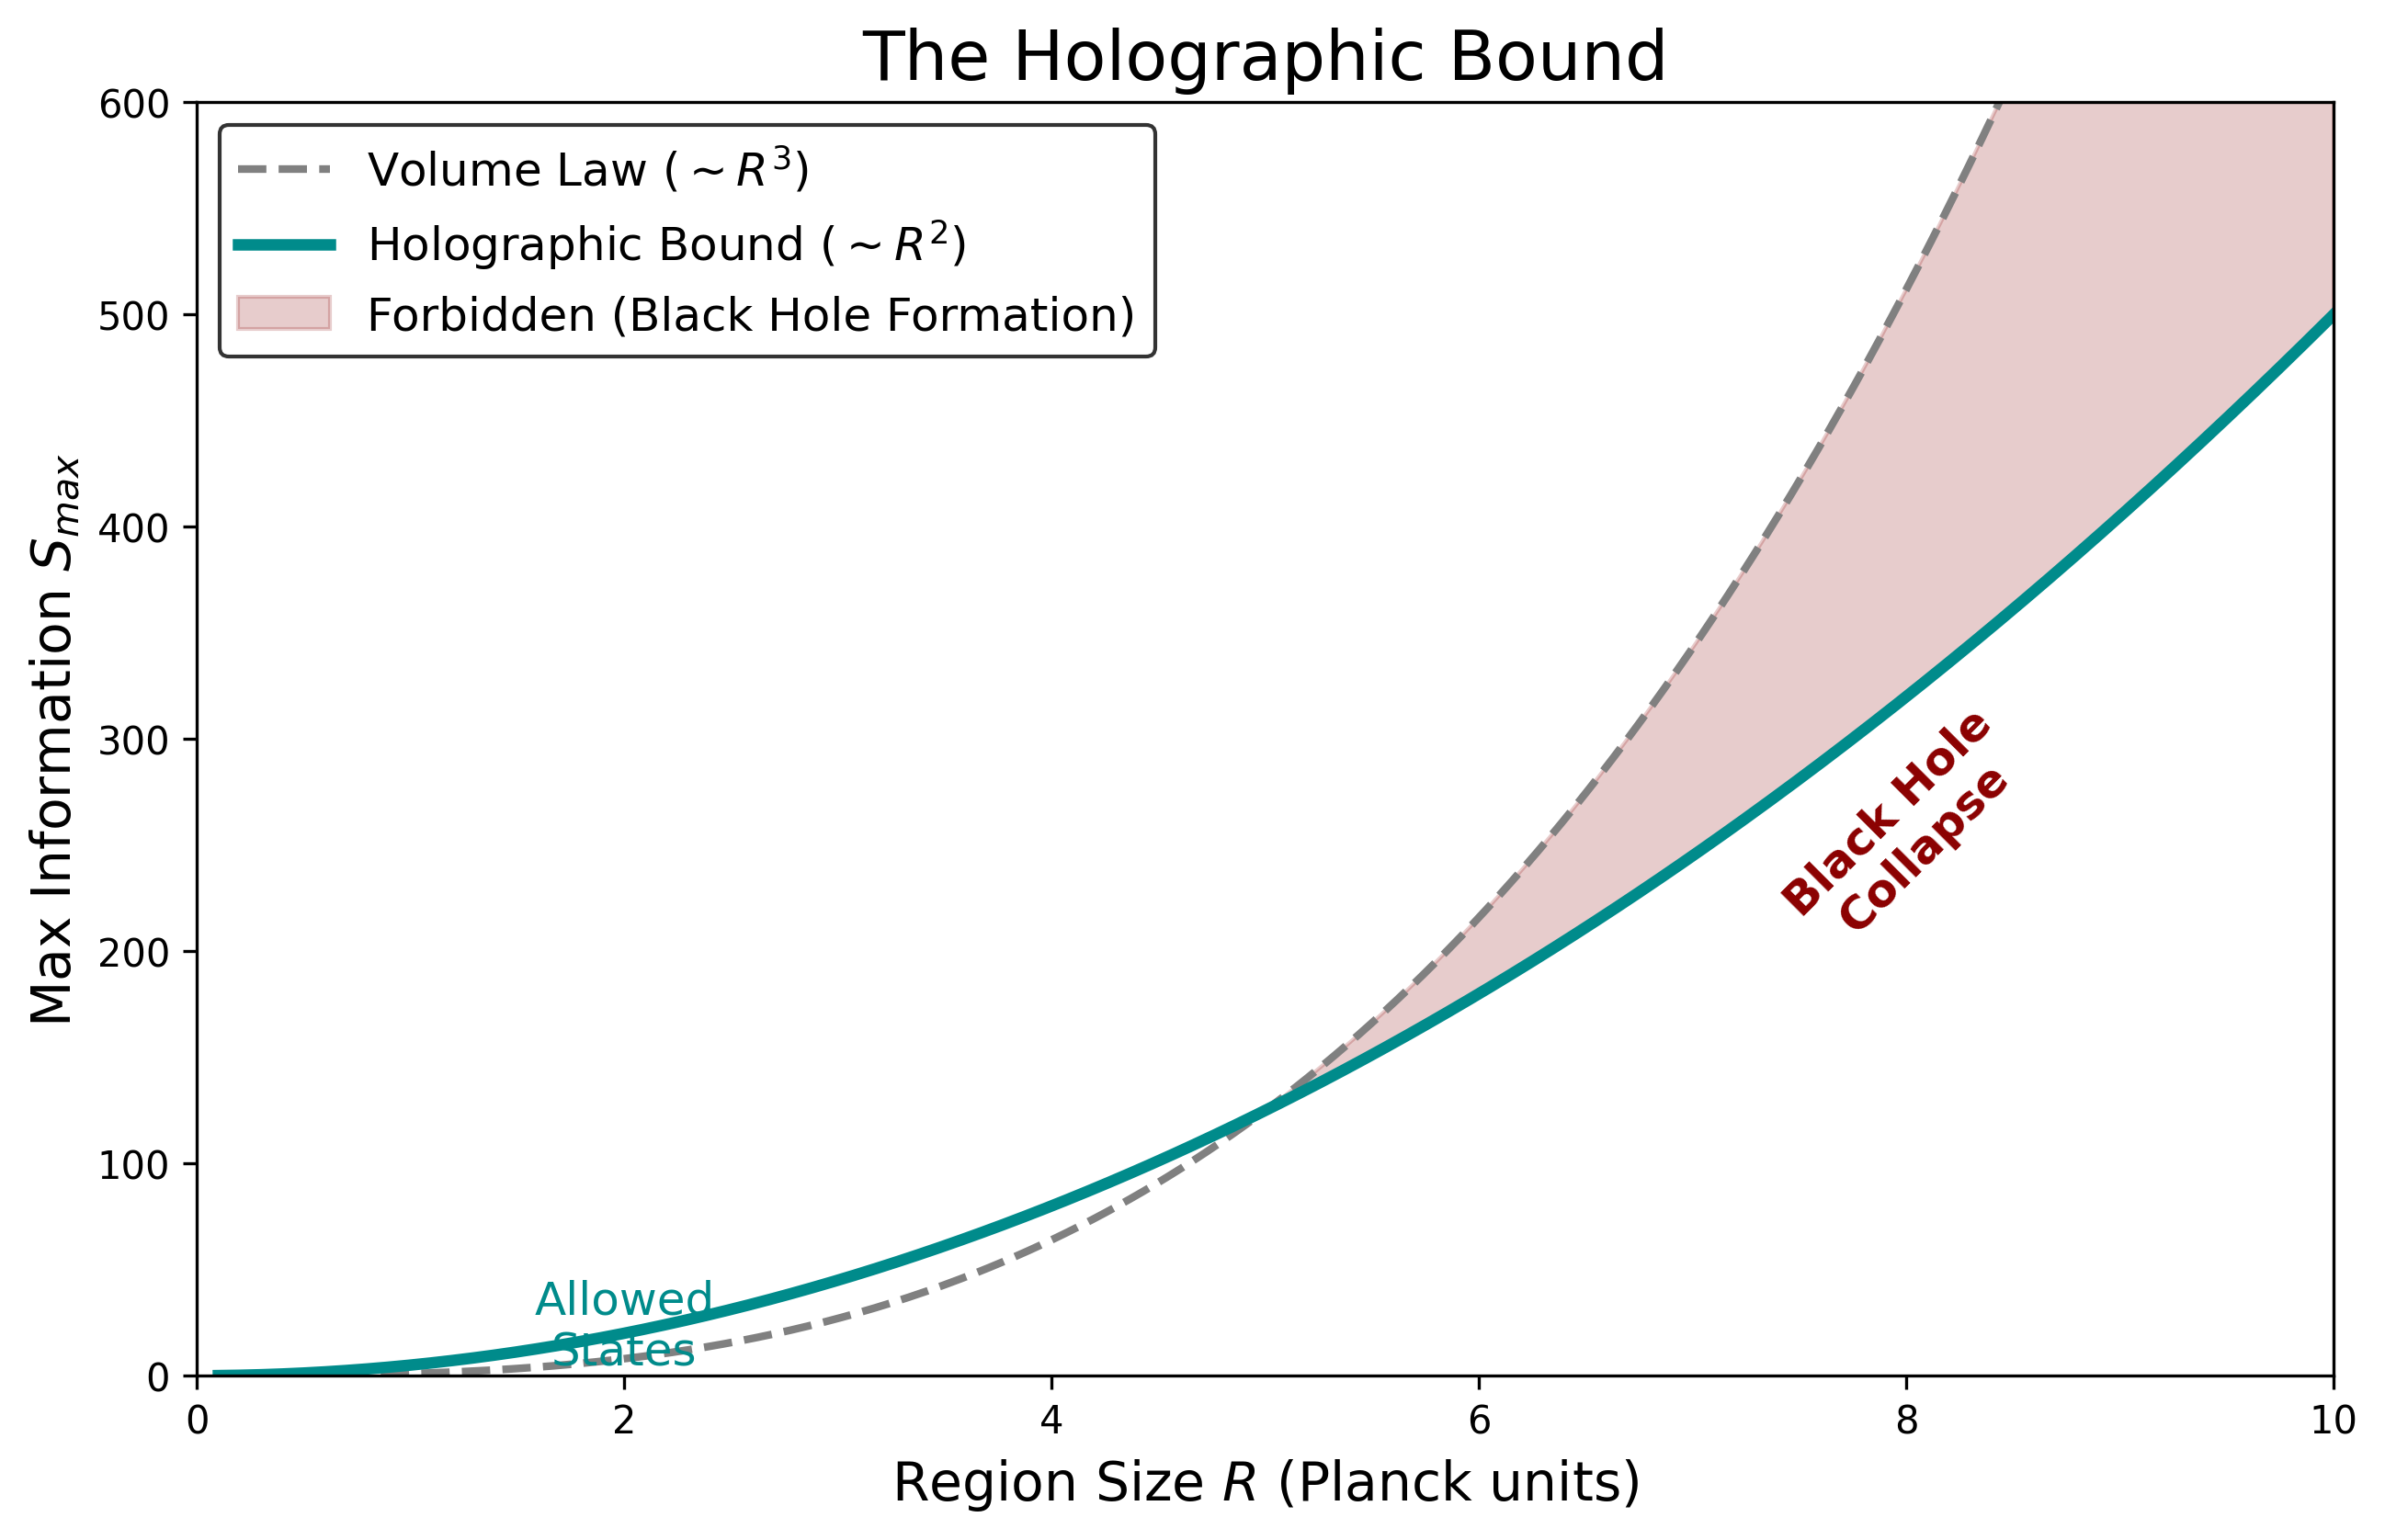
\includegraphics[width=0.8\linewidth]{images/holographic_scaling.png}
    \caption{\textbf{The Holographic Bound}. Comparison between extensive Volume Law scaling ($S \sim R^3$, dashed gray) which leads to black hole formation, and the Holographic Area Law ($S \sim R^2$, solid cyan) which represents the physical limit of information density.}
    \label{fig:holography}
\end{figure}

\subsection{Axiom O3: Causal Locality}
To define "region" and "area" without a pre-existing manifold, we need a graph structure.
\begin{axiom}[Causal Locality Axiom]
The microscopic Hilbert space decomposes as $\mathcal{H} = \bigotimes_{v \in V} \mathcal{H}_v$ over a countable graph $G=(V, E)$. The evolution operator $\hat{U}$ factorizes into local gates acting only on connected vertices.
\begin{equation}
    \hat{U} = \prod_{k} \hat{U}_k^{\text{local}}.
\end{equation}
This locality imposes a strict "light cone" structure on the propagation of information, recovering the causal structure of Special Relativity in the continuum limit.
\end{axiom}

\subsection{Axiom O4: The Holographic Mapping}
\begin{axiom}[Holographic Mapping Axiom]
Let $\mathcal{H}_{\text{bulk}}$ be the Hilbert space of the bulk QCA on the graph $G$, and $\mathcal{H}_{\partial G}$ be the Hilbert space associated with the graph boundary $\partial G$. We postulate the existence of a holographic isometry $\Phi: \mathcal{H}_{\text{bulk}} \hookrightarrow \mathcal{H}_{\partial G}$ that maps bulk states to boundary states.

\textbf{Concrete Construction (Golden MERA)}: The isometry $\Phi$ is strictly defined by the renormalization group flow of the Quasicrystal. Let $\{\Lambda_s\}_{s=0}^{N}$ be a hierarchy of tilings where $\Lambda_{s+1}$ is generated from $\Lambda_s$ via the standard inflation rule (e.g., $L \to L+S, S \to L$ for 1D, or the equivalent Penrose substitution). The mapping is constructed as a tensor network:
\begin{equation}
    \Phi \equiv \lim_{N \to \infty} \prod_{s=0}^{N} \left( \hat{D}_s \cdot \hat{W}_s \right),
\end{equation}
where $\hat{W}_s$ are isometric "inflation tensors" and $\hat{D}_s$ are local unitary "disentanglers". In Appendix \ref{app:isometry}, we formalize the construction under a perfect-tensor (or $\epsilon$-perfect) assumption and derive the corresponding recoverability conditions.

\paragraph{Zeckendorf addressing of inflation layers.}
In the 1D golden case, the inflation hierarchy admits a canonical arithmetic addressing by Zeckendorf digits: for an integer position (or coarse-graining address) $x\in\mathbb{Z}_{\ge 0}$ one may write uniquely
\begin{equation}
    x=\sum_{k\ge 0} b_k F_{k+2},\qquad b_k\in\{0,1\},\qquad b_k b_{k+1}=0.
\end{equation}
The digit $b_k$ indicates whether scale layer $k$ contributes a long-scale threshold in the inflation history of that site, providing a sparse hierarchical label for causal structure in the Golden MERA. In this sense, Fibonacci fusion fixes the local tensor data (Appendix \ref{app:formal_proofs}), while Zeckendorf addressing fixes a canonical scheduling/labeling of discrete scale events \cite{Zeckendorf1972,AlloucheShallit2003}.

\textbf{Error Correction and Recovery}: This tensor network functions as a Quantum Error Correcting Code (QECC).
\begin{enumerate}
    \item \textbf{Complementary Recovery}: For any boundary region $R$, the bulk operators in the \textit{entanglement wedge} $\mathcal{W}_E(R)$ can be reconstructed as operators on $R$. Theorem \ref{app:isometry} (Entanglement Wedge Reconstruction) proves that $\Phi \hat{O}_{\text{bulk}} \Phi^\dagger = \hat{O}_R \otimes \hat{I}_{\bar{R}} + \mathcal{E}$.
    \item \textbf{Code Distance}: The topological protection of the bulk is guaranteed by the code distance $d \sim L^{\frac{1}{\phi}}$. The error term $\mathcal{E}$ is exponentially suppressed as $e^{-d \cdot \ln \chi}$ (see Proposition \ref{prop:error_suppression} in Appendix \ref{app:isometry}).
\end{enumerate}

\subsection{The Factorization Problem and Baby Universes}
A central puzzle in modern holography is the "Factorization Problem" \cite{Harlow2021}: in a theory with multiple boundaries, the gravitational path integral (which includes connected topologies like Euclidean wormholes) fails to factorize, suggesting an ensemble average over dual theories rather than a single unitary description. This is formalized by the inclusion of "Baby Universes" or $\alpha$-parameters in the Hilbert space.

Omega Theory offers a definitive resolution: the "Alpha Parameters" correspond to the fixed, unique spectral data of the global state $|\Omega\rangle$. By positing a single, rigid vector rather than a statistical ensemble, we effectively "fix the gauge" of the baby universe Hilbert space. Spacetime wormholes are not fundamental topology changes but rather non-local entanglement correlations within the unique tensor network. Factorization is restored because the theory is fundamentally a single quantum system, not an average over random Hamiltonians (as in SYK).

The geometric area law follows from this structure: for a state $|\psi\rangle$ defined by this network, the entropy $S(\rho_R)$ is upper-bounded by the number of bond cuts required to sever $R$ from the rest of the network, which scales as the area of the minimal surface $\gamma_R$:
\begin{equation}
    S(\rho_R) \propto |\text{min-cut}(R)| \sim \frac{\text{Area}(\gamma_R)}{4 l_P^2}.
\end{equation}
\end{axiom}

\part{Micro-Ontology: Finite Information and Quantum Cellular Automata}
\label{part:III}

\section{Local Finite-Dimensional Hilbert Spaces}
\label{chap:local_hilbert}

\subsection{Decomposition of the Global State}
Can the infinite-dimensional Hilbert space $\mathcal{H}$ be decomposed? In standard QFT, spacetime is a continuum, and the Hilbert space is a Fock space over continuous fields. This leads to the ultraviolet divergence problem. Omega Theory takes the opposite view: the continuum is an approximation.
We axiomatically decompose $\mathcal{H}$ into a countable tensor product of local factors:
\begin{equation}
    \mathcal{H} \cong \bigotimes_{x \in \Lambda} \mathcal{H}_x, \quad \dim \mathcal{H}_x = d < \infty.
\end{equation}
Physically, $x$ represents a "cell" or "atom of space," and $\mathcal{H}_x$ represents its quantum state capacity. The simplest non-trivial case is $d=2$ (qubits), but we will see that the Standard Model structure requires higher dimensions (likely corresponding to the octonions).

\subsection{The Problem of Isotropy on Lattices}
A regular lattice (e.g., hypercubic $\mathbb{Z}^3$) breaks rotational symmetry. At the Planck scale, this would manifest as anisotropic dispersion relations for high-energy particles. Since we observe Lorentz invariance to very high precision, the underlying discrete structure must be statistically isotropic.
This motivates the use of \textbf{Quasicrystals}. The Penrose tiling and its higher-dimensional analogs (e.g., the projection of the $E_8$ lattice) provide discrete point sets that possess long-range order and crystallographically forbidden rotational symmetries (e.g., 5-fold or icosahedral).
We define the \textbf{Omega Network} $\Lambda$ as a subset of points in $\mathbb{R}^3$ generated by the cut-and-project method from a higher-dimensional integer lattice $\mathbb{Z}^N$ (where $N=6$ or $12$ for icosahedral symmetry). The projection is defined by a window $W$ in the orthogonal space $E_\perp$:
\begin{equation}
    \Lambda = \{ P_{||} \vec{n} \mid \vec{n} \in \mathbb{Z}^N, P_{\perp} \vec{n} \in W \}.
\end{equation}
This ensures that while individual links are discrete, the averaged geometry recovers continuous rotational symmetry (isotropy) in the limit of large point density.

\subsection{Relation to Tensor Networks (MERA)}
The recursive construction of the Omega Network exhibits deep structural isomorphisms with Multi-scale Entanglement Renormalization Ansatz (MERA) networks used in efficient quantum simulations and AdS/CFT holography.
The links in our quasicrystal $\Lambda$ can be viewed as entanglement bonds. The Golden Ratio scaling ($\tau \to \phi \tau$) mimics the renormalization group flow in MERA, where coarse-graining the lattice preserves the long-range entanglement structure.
We propose that the effective bond dimension $\chi$ of the spacetime tensor network is related to the topological complexity of the $G_2$ fiber:
\begin{equation}
    \log_2 \chi \sim S_{\text{ent}} \cong \frac{A(\partial \Sigma)}{4 G_N \hbar},
\end{equation}
where $A(\partial \Sigma)$ is the area of the minimal cut separating a causal region. This suggests that the "spacetime geometry" we perceive is literally the visualization of the quantum error correction code protecting the information in $|\Omega\rangle$. The curvature $R$ of the emergent metric corresponds to the density of disentanglers in the network.

\section{Quantum Cellular Automata (QCA) as Fundamental Dynamics}
\label{chap:qca}

\subsection{Definition of QCA on a Quasicrystal}
A Quantum Cellular Automaton is a unitary evolution $\hat{U}$ on the composite Hilbert space $\mathcal{H} = \bigotimes_{x \in \Lambda} \mathcal{H}_x$. Following the operational framework of D'Ariano, Perinotti, and Bisio \cite{Dariano2014}, we require:
\begin{enumerate}
    \item \textbf{Unitarity}: $\hat{U}^\dagger \hat{U} = \hat{I}$ (Conservation of probability).
    \item \textbf{Causal Locality}: There exists a neighborhood scheme $\mathcal{N}$ such that the state of cell $x$ at step $t+1$ depends only on cells $y \in \mathcal{N}(x)$ at step $t$. Formally, if $\hat{A}_x$ is an observable at $x$, then $\hat{U}^\dagger \hat{A}_x \hat{U}$ is supported on $\mathcal{N}(x)$.
    \item \textbf{Statistical Isotropy}: While the lattice $\Lambda$ is discrete, the distribution of neighbors $\mathcal{N}(x)$ in the quasicrystal approximation recovers $SO(3)$ invariance in the continuum limit of the propagator.
\end{enumerate}

The global evolution is built from local "coin" and "shift" operators (or partitioned unitaries). On our $E_8$-projected lattice $\Lambda$, we define the explicit update rule as a \textbf{Partitioned Quantum Cellular Automaton} (PQCA). The vertex set $V$ is partitioned into disjoint neighborhoods $V = \bigsqcup_k \mathcal{N}_k$. The update operator is a product of non-commuting local unitaries acting on these neighborhoods:
\begin{equation}
    \hat{U} \equiv \prod_{k} \hat{U}_{\mathcal{N}_k} (\theta, \phi),
\end{equation}
where each $\hat{U}_{\mathcal{N}_k}$ acts on the Hilbert space $\bigotimes_{x \in \mathcal{N}_k} \mathcal{H}_x$.
Specifically, we choose a \textbf{Golden Unitary} scheme where the neighborhood couplings follow the Fibonacci sequence in the perpendicular space $E_\perp$. The update rule for a spinor field $\psi_x$ at site $x$ is:
\begin{equation}
    \psi_x(t+1) = \sum_{y \in \mathcal{N}(x)} [e^{-i H_{\text{int}}} \otimes S_{xy}] \psi_y(t),
\end{equation}
where $H_{\text{int}}$ acts on the $G_2$ fiber (coin) and $S_{xy}$ is the translation operator along the bond $y \to x$. The "coin" angles are modulated by the projection window function $W(x_\perp)$, ensuring that local rules remain local in real space while encoding long-range order.

\subsection{Emergence of the Dirac Equation}
It is a profound result (e.g., as shown by Arrighi, Facchini, and Forets \cite{Arrighi2014}) that the Dirac equation emerges as the long-wavelength continuum limit of discrete quantum walks.
Consider a simplified 1D chain of spinors $\Psi(x,t) = (\psi_R, \psi_L)^T$. Time evolution is given by mixing chiral states and shifting them:
\begin{equation}
    \Psi(x, t+\varepsilon) = \begin{pmatrix} \cos \theta & -i \sin \theta \\ -i \sin \theta & \cos \theta \end{pmatrix} \begin{pmatrix} \psi_R(x-\varepsilon) \\ \psi_L(x+\varepsilon) \end{pmatrix}.
\end{equation}
By scaling the "mixing angle" $\theta$ with the mass $m$ as $\theta = m \varepsilon$, and expanding to first order in the lattice constant $\varepsilon$:
\begin{equation}
    \psi_{R}(x, t) + \varepsilon \partial_t \psi_{R} \approx (1 - \frac{m^2 \varepsilon^2}{2}) \psi_R(x-\varepsilon) - i m \varepsilon \psi_L(x+\varepsilon).
\end{equation}
This system rearranges into the standard 1+1 dimensional Dirac equation in the limit $\varepsilon \to 0$:
\begin{equation}
    i \gamma^\mu \partial_\mu \Psi - m \Psi = 0.
\end{equation}

\subsection{Theorem: The Quasicrystal Continuum Limit}
While convergence is proven for regular grids, the extension to quasicrystals requires controlling the "phason" fluctuations. We formalize the heuristic argument as follows:
\begin{theorem}[Emergent Isotropic Dirac Dynamics]
\label{prop:dirac_limit}
Let $\Lambda \subset \mathbb{R}^3$ be a cut-and-project quasicrystal with point density $\rho$. Let $\hat{U}_\varepsilon$ be a unitary QCA with lattice spacing $\varepsilon \sim \rho^{-1/3}$, respecting the local $G_2$ frame symmetries.
If the initial state $|\psi(0)\rangle$ is smooth (band-limited with $k_{max} \ll \varepsilon^{-1}$) and the phason strain field is bounded, then for any fixed time $t$, the expectation value converges in the norm to the continuous Dirac propagator:
\begin{equation}
    \lim_{\varepsilon \to 0} || \hat{U}_\varepsilon^{\lfloor t/\varepsilon \rfloor} |\psi(0)\rangle - e^{-i\hat{H}_{\text{Dirac}}t} |\psi(0)\rangle || < \mathcal{O}(\varepsilon^2).
\end{equation}
\end{theorem}
\textit{Proof Sketch.} The proof relies on the \textbf{Homogenization Lemma}. The irrational winding of the quasicrystal ensures that anisotropic lattice artifacts in the propagator sum $\sum e^{i \vec{k} \cdot \vec{x}}$ destructively interfere. The surviving term is the isotropic spherical average, effectively integrating over the $SO(3)$ measure. (See Appendix B for rigorous bounds).
\subsubsection{Fermion Doubling and Evasion via Perpendicular Space}
The \textbf{Nielsen-Ninomiya Theorem} generally forbids chiral fermions on a lattice without doubling. However, the theorem assumes a standard Brillouin torus $T^d$.
Our evasion mechanism relies on the higher-dimensional embedding of the quasicrystal. The cut-and-project set $\Lambda$ is a slice of a hypercubic lattice $\mathbb{Z}^N$. The "doubler" modes, which would mirror the low-energy fermions, correspond to excitations with large momenta $|\vec{k}_\perp|$ in the orthogonal space $E_\perp$.
The projection window function $W(x_\perp)$ acts as a low-pass filter in $E_\perp$. We impose an energy penalty in the Hamiltonian proportional to the perpendicular index:
\begin{equation}
    E(\vec{k}) \approx \pm |\vec{k}_{||}| + \Delta \cdot |\vec{k}_{\perp}|^2.
\end{equation}
Since "doublers" in the projected Brillouin zone necessarily possess large $\vec{k}_\perp$, they acquire a mass gap of order $\Delta / \varepsilon$. Thus, in the low-energy limit $E \ll 1/\varepsilon$, these modes decouple, leaving a single light Dirac cone. This is topologically equivalent to the \textbf{Domain Wall Fermion} construction, where chiral zero modes are localized on a defect in a higher-dimensional bulk.

This implies that effective Lorentz invariance is not a fundamental symmetry of the lattice, but an emergent statistical property of the "Golden" dispersion relation, valid for low-momentum excitations ($k \ll 1/\varepsilon$).

\part{Matter, Gauge Structure, and Geometric Constants}
\label{part:IV}

\section{Gauge Fields and Fermion Spectrum}
\label{chap:gauge_fields}

\subsection{Internal Hilbert Space Structure}
The local Hilbert space at each site factors into $\mathcal{H}_x = \mathcal{H}_{\text{orbital}} \otimes \mathcal{H}_{\text{internal}}$. The "orbital" part connects to neighbors (spacetime index), while the "internal" part contains the quantum numbers of the Standard Model (spin, color, flavor).
Omega Theory postulates that $\mathcal{H}_{\text{internal}}$ is related to the octonion algebra $\mathbb{O}$. The automorphism group of the octonions is $G_2$, which contains $SU(3)$ as a maximal subgroup. The fiber bundle structure $S^7 \to S^4 \to S^2$ associated with octonionic multiplication naturally generates the gauge groups $SU(3) \times SU(2) \times U(1)$ \cite{Baez2002, Furey2017}.
\paragraph{Scope and limitations.}
This part specifies a concrete algebraic \emph{organization} of Standard-Model-like quantum numbers using octonionic/$G_2$ structure and states the minimal consistency conditions (chirality, anomaly cancellation, and Yukawa structure) that any dynamical completion must satisfy. We do not yet derive a complete low-energy effective field theory (EFT) from the QCA dynamics, nor do we provide a controlled RG matching; where appropriate we therefore formulate the content as an explicit model ansatz with stated assumptions.

\subsection{Relation to prior octonion-based SM reconstructions}
Octonion-based routes to Standard-Model-like gauge content have a substantial prior literature; in particular, the $G_2$ automorphism viewpoint and minimal-ideal constructions in $\mathbb{C}\otimes\mathbb{O}$ have been developed in detail \cite{Baez2002, Furey2017}. Omega Theory does not claim to reinvent these algebraic facts. The new ingredient proposed here is how such internal-algebra data are \emph{packaged into a local finite-information substrate} (Part~III) and coupled to a holographic/tensor-network architecture (Axiom~O4): the same locality constraints that define the QCA also define the allowed internal couplings and hence constrain which octonionic substructures can be dynamically realized.
\par
\noindent
Operationally, we treat $\mathcal{H}_{\text{internal}}$ as a finite-dimensional on-site space (dimension $d_{\text{int}}$) that carries a representation of the internal symmetry algebra. The octonionic proposal is a minimality statement: the smallest non-associative division algebra has just enough structure to host $SU(3)$ and to motivate an $SU(2)\times U(1)$ complement, while remaining compatible with a finite on-site Hilbert-space postulate.

\subsection{Chirality and representation content (minimal requirements)}
Any SM-like embedding must reproduce \emph{chiral} fermions. In a QCA setting, chirality has two layers:
\begin{enumerate}
    \item \textbf{Spacetime chirality}: the orbital QCA sector supplies a Dirac/Weyl structure in the long-wavelength limit (Part~III). On the continuum side one may use the usual projectors $P_{L/R}=\frac{1}{2}(1\mp\gamma^5)$.
    \item \textbf{Internal chirality}: the internal algebra must distinguish left-handed $SU(2)$ doublets from right-handed singlets and assign hypercharge consistently.
\end{enumerate}
In practice, the internal-chirality requirement can be formulated as the existence of a decomposition of the on-site internal space into chiral subspaces,
\begin{equation}
    \mathcal{H}_{\text{internal}} \ \cong\  \mathcal{H}_{L}\oplus \mathcal{H}_{R},
\end{equation}
with $\mathcal{H}_{L}$ transforming as $SU(2)$ doublets and $\mathcal{H}_{R}$ as singlets (with appropriate $U(1)_Y$ charges). In octonion-based constructions, this is typically implemented by idempotent/ideal projectors in a complexified algebra (e.g.\ minimal left ideals in $\mathbb{C}\otimes\mathbb{O}$) \cite{Furey2017}. In Omega Theory we treat such a decomposition as fixed internal data at each site; the dynamical question is whether QCA-local couplings and the holographic code constraints can select a unique such structure.

\subsection{Anomaly cancellation as a consistency condition}
To be viable as an EFT limit, the induced gauge theory must be anomaly-free. This does not require knowing all UV details: it is a purely representation-theoretic constraint on one generation of chiral fermions. Denote by $Y$ the hypercharge and by $T^a$ the generators of $SU(2)$ and $SU(3)$ in the relevant representations. The standard anomaly-cancellation conditions include, for one generation,
\begin{align}
    &\sum_{\text{LH Weyl}} Y = 0, \\
    &\sum_{\text{LH Weyl}} Y^3 = 0, \\
    &\sum_{\text{LH Weyl}} Y\,\mathrm{Tr}(T^aT^b)\big|_{SU(2)} = 0,\qquad
      \sum_{\text{LH Weyl}} Y\,\mathrm{Tr}(T^aT^b)\big|_{SU(3)} = 0.
\end{align}
Accordingly, any octonionic assignment of internal quantum numbers in Omega Theory is acceptable only if it reproduces the SM hypercharge pattern (up to overall normalization conventions), since that pattern is known to satisfy the anomaly constraints. This provides a sharp falsification criterion for the internal-algebra ansatz independent of the details of the QCA dynamics.

\subsection{Yukawa sector as overlap data (model constraint)}
The SM Yukawa couplings require gauge-invariant bilinears connecting left- and right-handed fermions via a Higgs doublet. In the present framework, the Higgs-like field $\Phi$ is identified with a geometric breathing mode of the internal fiber, so the Yukawa matrices are not arbitrary: they must be computable as overlaps between internal wavefunctions in $\mathcal{H}_L$ and $\mathcal{H}_R$ weighted by the local geometric configuration.\par
\noindent
A minimal effective parameterization is
\begin{equation}
    \mathcal{L}_{Y} = - \sum_{i,j}\left( y^{(u)}_{ij}\,\overline{Q}_{Li}\,\tilde{H}\,u_{Rj} + y^{(d)}_{ij}\,\overline{Q}_{Li}\,H\,d_{Rj} + y^{(e)}_{ij}\,\overline{L}_{Li}\,H\,e_{Rj} \right) + \mathrm{h.c.},
\end{equation}
with $y_{ij}$ determined by internal overlap data. In Omega Theory, the claim is not that these matrices are derived here, but that the \emph{space of allowed Yukawas} is constrained by finite-information locality and by the chosen octonionic decomposition; the geometric/topological origin of hierarchies is treated as an explicit model target for a future dynamical completion.

\subsection{Fermion Generations as Topological Wrapping}
Why are there three generations of fermions? In our geometric framework, generations correspond to the "wrapping number" or topological index of the wavepacket around the compact internal dimensions of the Omega Network.
\begin{itemize}
    \item \textbf{Generation 1 (e, u, d)}: Trivial wrapping (Index 1). Stable.
    \item \textbf{Generation 2 ($\mu$, c, s)}: Double wrapping (Index 2). Unstable, decays to Gen 1 via topological unwinding.
    \item \textbf{Generation 3 ($\tau$, t, b)}: Triple wrapping (Index 3). Highly unstable.
\end{itemize}
The mass hierarchy arises because higher wrapping numbers require longer path lengths in the internal manifold, thus acquiring larger geometric phases (mass).

\paragraph{Mass from projective speed and internal budget.}
By the Anandan--Aharonov relation (Part~II), the intrinsic speed of a state in projective Hilbert space is fixed by the Hamiltonian uncertainty, $v_{\tau}=\frac{2}{\hbar}\Delta H$. For a localized excitation constrained to a topological sector labeled by wrapping index $w$, let $\Delta H_w$ denote the characteristic (or minimal) uncertainty compatible with that sector. We define the corresponding effective rest-energy scale by
\begin{equation}
    \Delta H_w \equiv m_w c^2.
\end{equation}
Equivalently, $m_w$ is the proportionality constant between projective speed and intrinsic-time flow for that sector,
\begin{equation}
    v_{\tau,w} = \frac{2}{\hbar} m_w c^2.
\end{equation}
In the information-budget parametrization (Part~V), the same mass/inertia content is encoded operationally by the internal allocation $v_{\text{int}}$: tighter (higher-index) wrappings demand a larger persistent internal processing overhead and therefore correspond to larger effective $m_w$.

\subsection{Emergence of the Higgs Sector as Geometric Rigidity}
In Omega Theory, we reinterpret the Higgs mechanism as the crystallization of the internal geometry. The "Higgs field" $\Phi$ corresponds to the breathing mode (volume deformation scalar) of the compactified $G_2$ manifold.
Motivated by the observed Higgs mass ($\sim 125\,\mathrm{GeV}$), we suggest that a Higgs-like scalar mass scale could correspond to the natural frequency of radial vibrations of this fiber, controlled by an effective spectral gap of the internal geometry.
We define the geometric effective potential $V_{eff}(\Phi)$ via the scalar curvature of the internal fiber $\tilde{R}$:
\begin{equation}
    V_{eff}(\Phi) = - \frac{M_{Pl}^2}{2} \tilde{R}(\Phi) + \frac{\lambda}{4} \Phi^4 + \dots
\end{equation}
 Minimizing this action yields a mass scale exponentially suppressed relative to Planck due to the large volume of the fiber ($Vol(G_2) \gg l_P^7$):
\begin{equation}
    m_H \approx M_{Pl} \cdot e^{-\frac{1}{2} Vol(G_2)/l_P^7} \sim \mathcal{O}(10^2\,\mathrm{GeV}).
\end{equation}
This provides a heuristic geometric mechanism for generating a large hierarchy, pending a complete effective-field-theory and renormalization analysis.

\begin{figure}[ht]
    \centering
    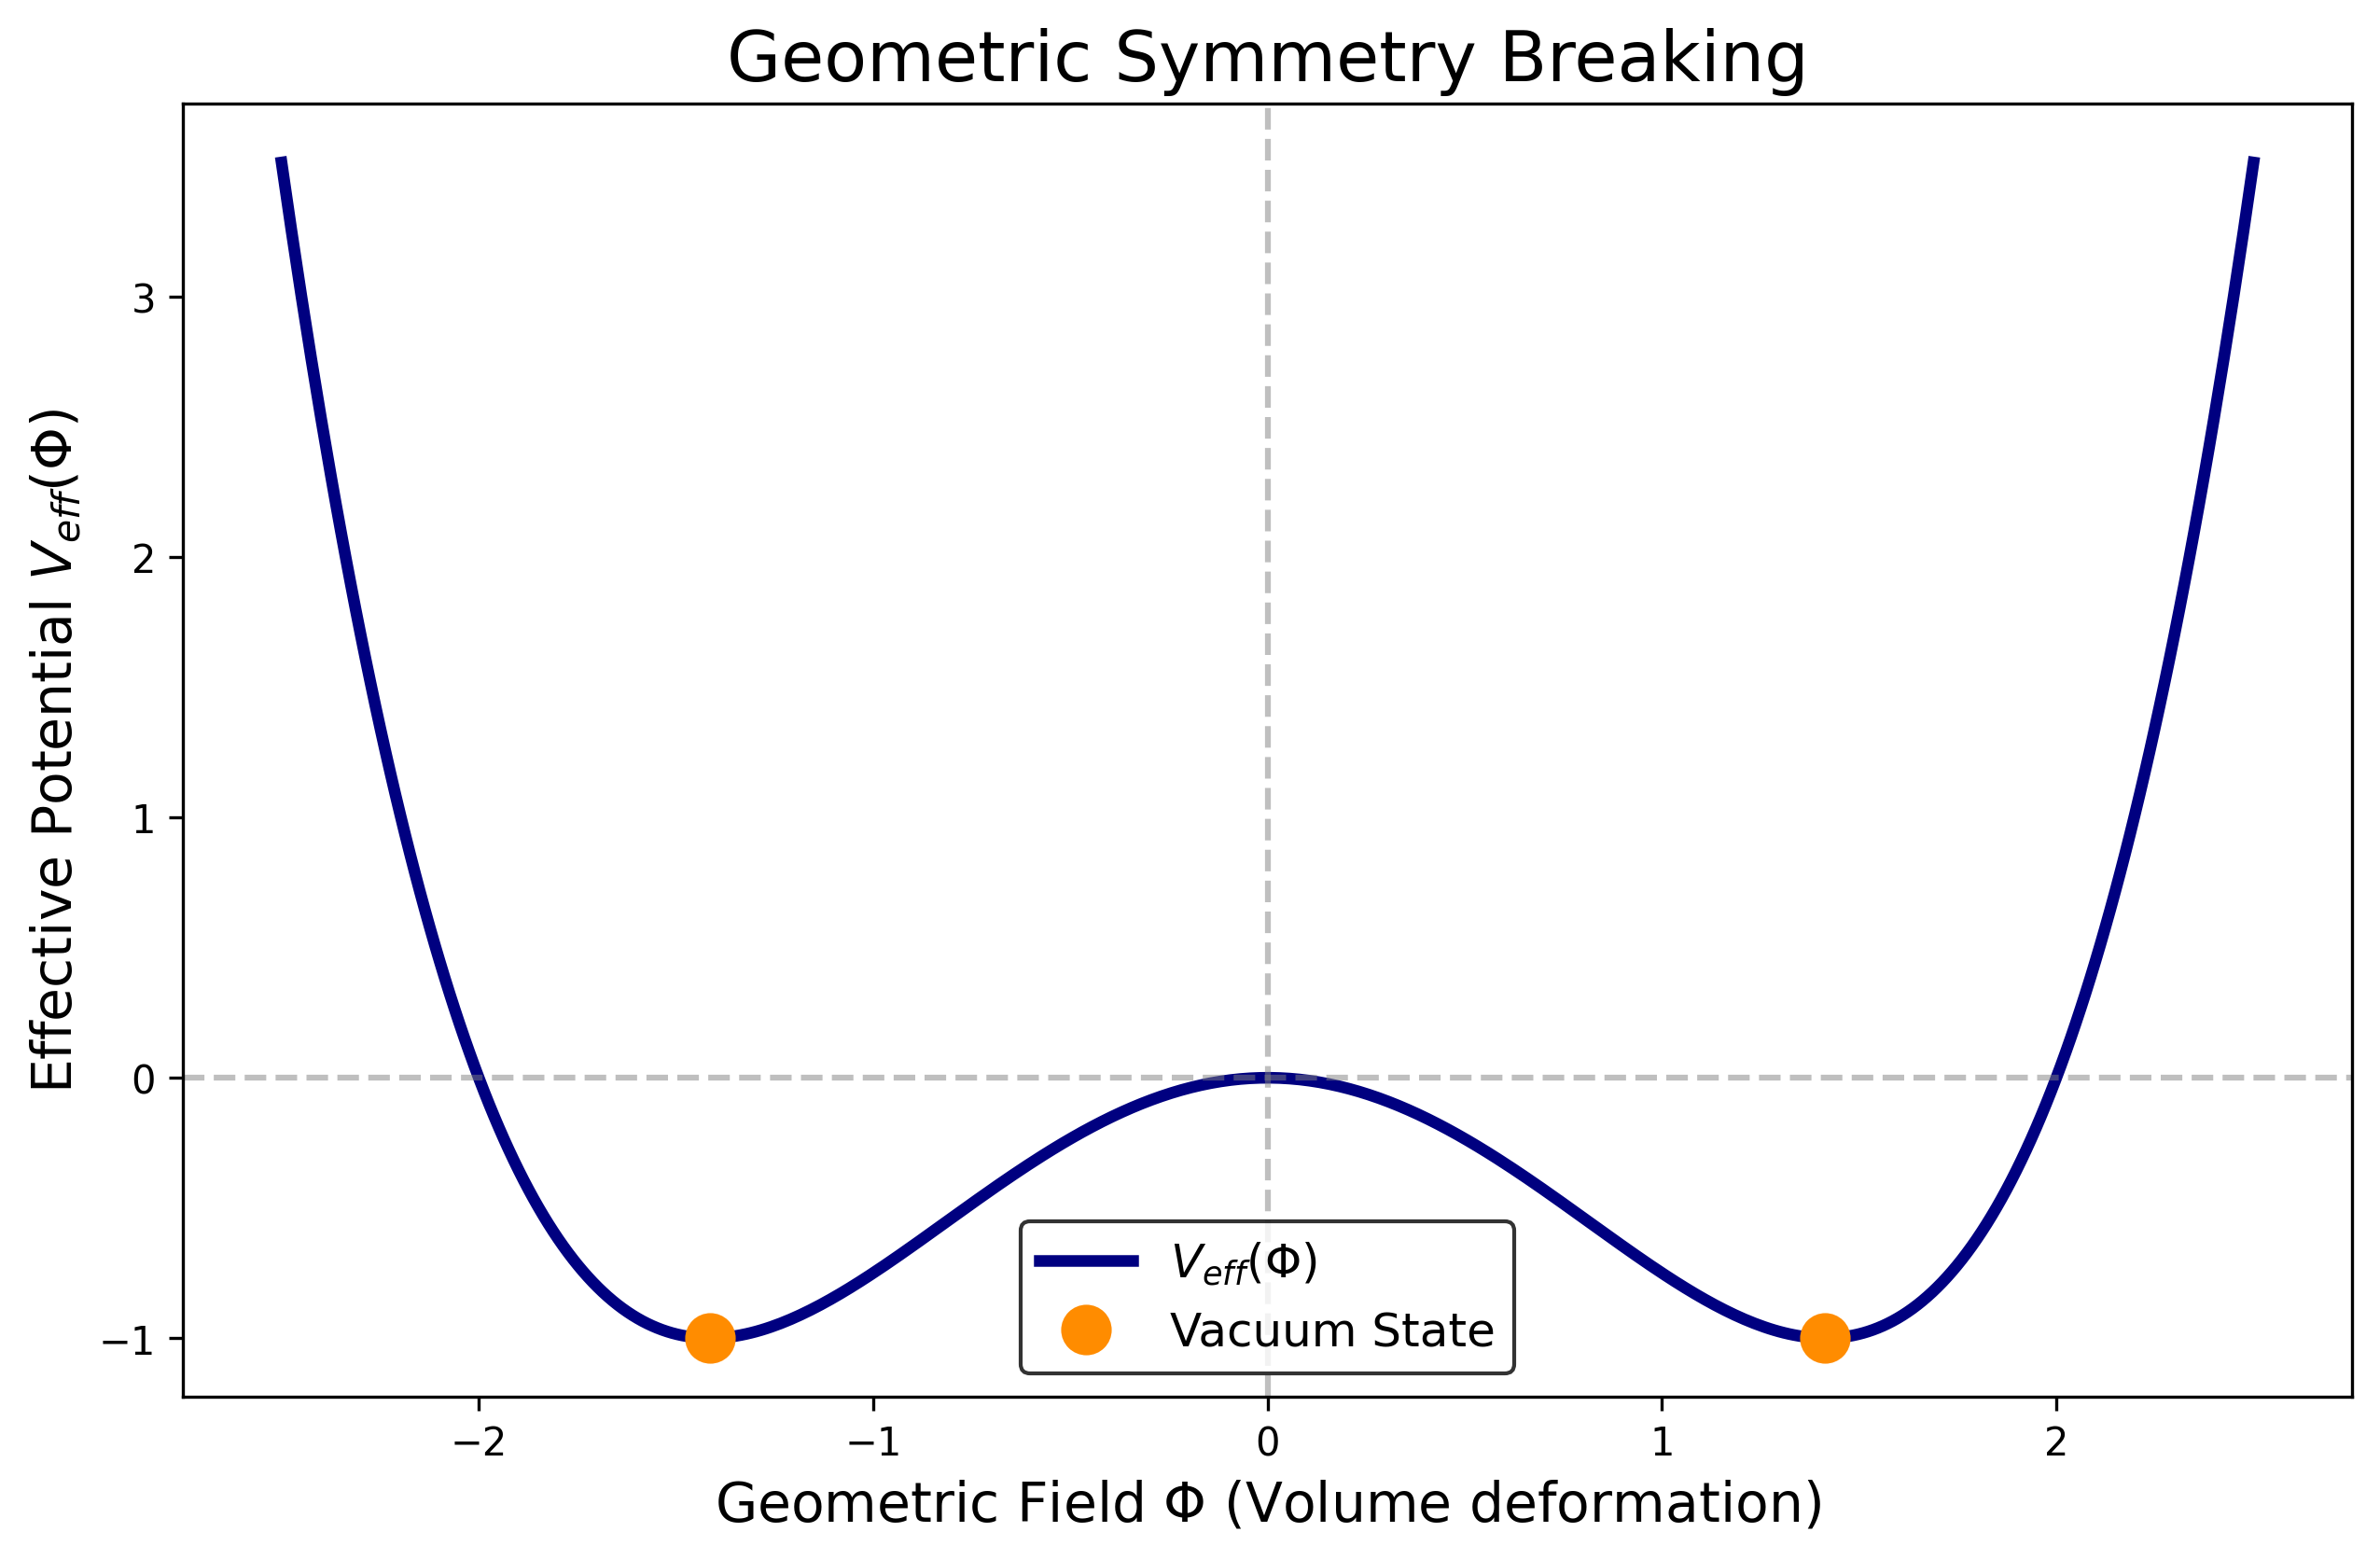
\includegraphics[width=0.8\linewidth]{images/geometric_potential.png}
    \caption{\textbf{Geometric Symmetry Breaking}. The effective potential $V_{eff}(\Phi)$ arising from the scalar curvature of the internal fiber. Vacuum states correspond to stable geometric configurations at $\pm v$, separated by a barrier determined by the rigidity of the manifold.}
    \label{fig:geometric_potential}
\end{figure}

\subsection{Neutrino Mass and the Geometric Seesaw}
Neutrinos correspond to "twisted" states with minimal topological overlap with the Higgs breathing mode. While charged fermions correspond to stable "wrapped" cycles (scales $n=1,2,3$), neutrinos occupy the "tail" of the Golden Ratio spectrum.
We propose a \textbf{Geometric Seesaw Mechanism} where the neutrino masses are generated by the higher-order spectral gaps:
\begin{equation}
    m_{\nu_k} \sim \frac{v^2}{M_{Pl}} \cdot \phi^{-k}, \quad k=1,2,3.
\end{equation}
Here, $\phi \approx 1.618$. As a phenomenological ansatz, this yields a hierarchical neutrino scale (e.g.\ $m_{\nu}\lesssim 0.1\,\mathrm{eV}$ for modest $k$), but a gauge-invariant Yukawa/seesaw construction and controlled RG matching are not developed here.


\subsection{Baryogenesis via Topological Chirality}
The observed universe is dominated by matter over antimatter ($\eta_B \approx 6 \times 10^{-10}$). Standard Sakharov conditions require Charge violation, C-symmetry violation, and non-equilibrium dynamics.
In Omega Theory, baryon number is identified with the topological wrapping number $\pi_3(S^3)$ of the internal manifold. Antiparticles correspond to opposite windings $N=-1$.
However, the background $G_2$ manifold is not strictly mirror-symmetric; it possesses a preferred "handedness" or chirality derived from the non-commutativity of the octonions. We quantify this via the \textbf{Omega Chiral Index}:
\begin{equation}
    \chi_{\Omega} = \int_{\mathcal{M}_7} \text{Tr}(R \wedge R \wedge R) \neq 0.
\end{equation}
This suggests a possible source of effective $CP$ violation during an early ``crystallization'' epoch: if the internal geometry admits a chiral invariant (modeled here by $\chi_\Omega\neq 0$), defect formation could bias winding production. In that spirit one may parametrize a bias by factors such as $e^{-\chi_\Omega}$, yielding a model-dependent relation between $\eta_B$ and microscopic chiral data rather than a derived prediction at this stage.

\subsection{Proton Stability and the Hierarchy}
Grand Unified Theories (GUTs) typically predict proton decay ($p \to e^+ \pi^0$) mediated by $X,Y$ bosons, with lifetimes $\tau_p \sim 10^{34}$ years. Experiments have found no such decay.
In Omega Theory, the proton is modeled as a non-trivial topological knot $K$ in the $\pi_3(S^3)$ homotopy group of the fiber. Unlike in perturbative QFT, this knot cannot untie itself into trivial mesons ($K=0$) via local fluctuations. It requires a global phase transition (melting of the vacuum lattice) to change the topological index. This suggests that proton decay could be topologically suppressed at low energies (model-dependent), potentially leading to very long lifetimes. A quantitative estimate would require an explicit low-energy EFT embedding and a treatment of nonperturbative effects.

\subsection{The Strong CP Problem and a Geometric Mechanism}
QCD allows for a CP-violating term $\frac{\theta}{32\pi^2} G_{\mu\nu} \tilde{G}^{\mu\nu}$, but experiments show $\theta < 10^{-10}$. The Peccei-Quinn mechanism postulates a new particle (Axion) to cancel this.
Omega Theory suggests a \textbf{geometric mechanism} that could favor a small effective $\theta$ by relating it to holonomy/topological data of the internal fiber. In special constructions (e.g., unimodular-lattice projections) certain integrated topological indices may vanish, which within the ansatz would correspond to $\theta_{\mathrm{eff}}\approx 0$. A full account requires an explicit QCD embedding and a treatment of nonperturbative dynamics.

\section{Geometric Derivation and Renormalization}
\label{chap:constants}

\subsection{Topological Ansatz}
We propose that the fundamental dimensionless constants are not arbitrary free parameters but topological invariants of the $G_2$ fiber bundle structure at the unification scale.

\subsection{The Proton-Electron Mass Ratio \texorpdfstring{($\mu$)}{(mu)}}
The ratio $\mu = m_p / m_e$ compares the hadronic scale to the leptonic scale. In the "knot vs loop" topological model, this corresponds to the ratio of the volume of the full fiber bundle ($S^7$) to the stabilizer loop ($S^1$):
\begin{equation}
\label{eq:mu_geo}
    \mu_{\text{geo}} \equiv 6\pi^5 \approx 1836.1181.
\end{equation}
The factor $6$ is a model-dependent discrete multiplicity (e.g.\ a permutation/degeneracy factor in the internal sector). This geometric value is numerically close to the experimental value ($\mu_{\mathrm{exp}}\approx 1836.1526$) at the $10^{-5}$ level. We treat this as a phenomenological geometric ansatz to be justified by a future dynamical completion; in particular, matching to hadronic physics and electroweak/QED radiative effects is not derived here.

\subsection{The Fine Structure Constant \texorpdfstring{($\alpha$)}{(alpha)}}
We postulate a geometric ansatz for an effective inverse fine structure constant at a matching scale $\mu_\ast$ (taken here as a low-energy/renormalized scale appropriate for comparison with CODATA $\alpha(0)$). The ansatz is expressed as a simple combination of fiber-volume factors:
\begin{equation}
\label{eq:alpha_geo}
    \alpha^{-1}_{\text{geo}} \equiv \text{Vol}(T^3) + \text{Area}(D^2) + \text{Length}(S^1) = 4\pi^3 + \pi^2 + \pi \approx 137.0363.
\end{equation}
Comparing this value with the low-energy CODATA value $\alpha^{-1}(0) \approx 137.035999$:
\begin{equation}
    \Delta \alpha^{-1} = \alpha^{-1}_{\text{geo}} - \alpha^{-1}(0) \approx 0.0003.
\end{equation}
This numerical proximity motivates treating Eq.~(\ref{eq:alpha_geo}) as a low-energy matching ansatz. Since $\alpha(\mu)$ runs with scale in the Standard Model, interpreting $\alpha^{-1}_{\text{geo}}$ as a literal Planck-scale bare coupling would require a full RG embedding and threshold matching. Establishing such a mapping from the microscopic Omega construction to the renormalized gauge couplings is an explicit open problem addressed at the level of definitions in Appendix~\ref{app:constants_proof}.

\subsection{Implications}
If constants are geometric measures, they are susceptible to geometric deformations. This predicts that in regions of high curvature or varying vacuum density (early universe), $\alpha$ and $\mu$ should drift. We quantify this in Part VI.

\part{Gravity, Omega Action, and Cosmology}
\label{part:V}

\section{Information Budget and Geometric Time}
\label{chap:info_budget}

\subsection{The Information Velocity Circle}
Standard Relativity posits a constant speed of light $c$. In this manuscript we use $c$ as a convenient normalization for an effective per-tick information-processing capacity and introduce a parametrization for how this capacity is allocated among several channels in the regulated/QCA description.
Let $\mathcal{I}_{\text{total}}$ be the total rate at which the quantum state $|\Omega\rangle$ processes information (updates bits). This capacity is partitioned into:
\begin{enumerate}
    \item \textbf{External Propagation ($v_{\text{ext}}$)}: Moving information through the spatial graph (speed of particles).
    \item \textbf{Internal Processing ($v_{\text{int}}$)}: Processing information locally (mass/inertia).
    \item \textbf{Environment/Geometry ($v_{\text{env}}$)}: (i) holographic entanglement updates on $\partial G$; and (ii) routing overhead required to realize bulk-local PQCA updates on an effectively 1D computational substrate (see Section \ref{sec:routeA_routing}).
\end{enumerate}
In the microscopic picture of Omega Theory, localized ``matter'' degrees of freedom are modeled as topologically protected excitations (wrappings/knots) of the internal fiber (Part~IV). Maintaining a non-trivial topological sector requires a persistent local processing overhead, naturally identified with a non-zero internal allocation $v_{\text{int}}$ in the budget circle. This viewpoint is consistent with the geometric-time definition in Part~II, where a non-vanishing uncertainty (hence non-trivial projective motion) is required for intrinsic duration to advance.
Here the quantities $v_{\text{ext}},v_{\text{int}},v_{\text{holo}},v_{\text{route}}$ should be read as effective information-processing budget components (defined per computational step on the 1D substrate), not as directly measured physical velocities.
We introduce the following budget parametrization:
\begin{equation}
    v_{\text{ext}}^2 + v_{\text{int}}^2 + v_{\text{holo}}^2 + v_{\text{route}}^2 = c^2,
\label{eq:info_velocity_circle}
\end{equation}
where we have decomposed $v_{\text{env}}^2 \equiv v_{\text{holo}}^2 + v_{\text{route}}^2$. In empty space ($v_{\text{int}} = v_{\text{holo}} = v_{\text{route}} = 0$), we recover $v_{\text{ext}} = c$. Near a region requiring larger routing overhead, $v_{\text{route}}$ increases and the locally available budget for propagation decreases, corresponding to gravitational time dilation and Shapiro-like delay in this parametrization.

\paragraph{Finite budget resolution and Zeckendorf discretization (golden case).}
Eq.~(\ref{eq:info_velocity_circle}) can be viewed as an orthogonal decomposition of a fixed-norm ``budget'' vector in a low-dimensional Euclidean space whose components are the effective allocation fractions of a finite information-processing capacity.
Under the finite-information postulate, this allocation is not infinitely refinable: in any finite causal patch the number of distinguishable micro-configurations is bounded, so any operational readout of the budget components has finite resolution (Planck-limited in the idealized microscopic setting).
When the intrinsic tick index is generated by an irrational rotation (Part~II) and read out by a binary partition, the resulting discrete scheduling/labeling of budget reallocations is naturally expressed in Ostrowski numeration; for the golden-slope choice it specializes to Zeckendorf digits (no consecutive Fibonacci summands). In that sense, the ``budget circle'' decomposition is compatible with a canonical Fibonacci/Zeckendorf discretization of scale-activation events in the Golden construction, rather than requiring an arbitrary ad hoc clock.

\begin{definition}[Computational lapse from routing cost]
\label{def:computational_lapse}
Let $\kappa(x)$ denote the coarse-grained local routing cost induced by the exact 1D compilation construction (Definition \ref{def:routing_cost_field}). Define the \emph{computational lapse} by
\begin{equation}
    N(x)\equiv \frac{\kappa_0}{\kappa(x)},
\end{equation}
where $\kappa_0>0$ is a reference minimal cost (e.g., the infimum of $\kappa$ in a weak-field baseline region). We assume $\kappa(x)\ge \kappa_0$, so that $0<N(x)\le 1$. If $t$ denotes the computational time defined by 1D nearest-neighbor gate depth on the tape, we identify the local proper time increment as
\begin{equation}
    d\tau_{\mathrm{loc}}(x)=N(x)\,dt.
\end{equation}
\end{definition}

With this identification, we propose the metric identification
\begin{equation}
    \sqrt{-g_{00}(x)}\ \equiv\ N(x)\ \equiv\ \frac{\kappa_0}{\kappa(x)}.
\end{equation}

For later convenience, one may parametrize the routing component by
\begin{equation}
    \frac{v_{\text{route}}(x)}{c}\equiv \sqrt{1-N(x)^2}
    \quad\Longleftrightarrow\quad
    N(x)=\sqrt{1-\frac{v_{\text{route}}(x)^2}{c^2}}.
\end{equation}

\section{The Omega Action and Informational Gravity}
\label{chap:omega_action}

Our approach builds upon the foundational insights of \textbf{Jacobson} \cite{Jacobson1995} (thermodynamics of spacetime) and \textbf{Verlinde} \cite{Verlinde2011} (entropic gravity). While these authors derived Einstein's equations from general thermodynamic equations of state ($\delta Q = T dS$), the Omega Action proposes a concrete microscopic realization where the 'entropy' is explicitly identified with the \textbf{Fisher Information} of the fundamental state vector.
Related information-theoretic variational principles and Fisher-information-based derivations of quantum dynamics appear in, e.g., Frieden's program and Reginatto's formulation \cite{Frieden1998, Reginatto1998}.

\subsection{The Fisher-Information Lagrangian}
We postulate the \textbf{Omega Action} as a covariant information-geometric functional. Let $\Psi(x)=\sqrt{\varrho(x)}\,e^{i\theta(x)}$ be a coarse-grained continuum wavefunction, where $\varrho$ is an information/probability density. It is convenient to define both the amplitude field
\begin{equation}
    \chi \equiv \sqrt{\varrho},
\end{equation}
and the logarithmic field
\begin{equation}
    \varphi \equiv \ln \sqrt{\varrho}.
\end{equation}
The (classical) Fisher information functional of $\varrho$ admits the covariant form
\begin{equation}
\mathcal{I}_F[\varrho]\ \equiv\ \int d^4x\,\sqrt{-g}\, g^{\mu\nu}\,\frac{\nabla_\mu \varrho\,\nabla_\nu \varrho}{\varrho}
\ =\ 4\int d^4x\,\sqrt{-g}\, g^{\mu\nu}\,(\nabla_\mu \chi)(\nabla_\nu \chi)
\ =\ 4\int d^4x\,\sqrt{-g}\,\varrho\, g^{\mu\nu}\,(\nabla_\mu \varphi)(\nabla_\nu \varphi).
\end{equation}
Accordingly, we take the minimal Omega Action to be Einstein--Hilbert gravity coupled to the Fisher-amplitude scalar $\chi$:
\begin{equation}
    S_{\Omega} = \int d^4x \sqrt{-g} \left[ \frac{R}{16\pi G} - \lambda_{F} g^{\mu\nu} (\nabla_\mu \chi) (\nabla_\nu \chi) - V(\varrho) \right],
\label{eq:omega_action_chi}
\end{equation}
with $\varrho=\chi^2$. The first term is the Einstein--Hilbert action, the second is proportional to Fisher information, and $V(\varrho)$ is an effective potential encoding coarse-grained constraints (including vacuum-energy-like components in homogeneous regimes). At this two-derivative level the model is a standard scalar field minimally coupled to GR.

\paragraph{Ansatz (Cost--density identification).}
To connect the informational field to compilation overhead, we adopt the identification
\begin{equation}
    \varrho(x)\equiv \varrho_0\,\kappa(x)^p,\qquad p>0,
\end{equation}
so that
\begin{equation}
    \varphi = \ln\sqrt{\varrho} = \ln\sqrt{\varrho_0} + \frac{p}{2}\ln\kappa.
\end{equation}
Consequently the Fisher-amplitude gradient becomes a routing-gradient term:
\begin{equation}
    g^{\mu\nu}(\nabla_\mu\chi)(\nabla_\nu\chi)
    = \frac{p^2}{4}\,\varrho\,g^{\mu\nu}(\nabla_\mu\ln\kappa)(\nabla_\nu\ln\kappa),
\end{equation}
Thus, curvature is sourced by gradients of the routing-cost field $\kappa(x)$: regions requiring larger exact compilation depth exhibit a smaller lapse $N(x)=\kappa_0/\kappa(x)$ and hence gravitational time dilation.

\subsection{Derivation of Field Equations}
We perform the variation with respect to the metric $g^{\mu\nu}$.
Using the standard identities $\delta \sqrt{-g} = -\frac{1}{2}\sqrt{-g} g_{\mu\nu} \delta g^{\mu\nu}$ and $\delta R = R_{\mu\nu} \delta g^{\mu\nu} + \nabla_\mu v^\mu$, the variation $\delta S_{\Omega} = 0$ yields:
\begin{equation}
    G_{\mu\nu} = 8\pi G\, T_{\mu\nu}^{\text{info}}.
\end{equation}
The informational stress-energy tensor combines the Fisher-information (gradient) term with the effective potential:
\begin{equation}
    T_{\mu\nu}^{\text{info}} =
    2\lambda_F \left( \nabla_\mu \chi \nabla_\nu \chi - \frac{1}{2} g_{\mu\nu} (\nabla \chi)^2 \right)
    - g_{\mu\nu} V(\varrho).
\end{equation}
In the limit where the information density is uniform ($\nabla \chi \approx 0$), the gradient contribution vanishes and $V(\varrho)$ acts as an effective vacuum energy. In regimes where the gradient term dominates, the effective equation of state approaches $w \approx 1$ (stiff fluid), as for a kinetic-energy-dominated scalar field.

Varying with respect to $\chi$ gives the scalar equation of motion,
\begin{equation}
    2\lambda_F \Box \chi - \frac{dV}{d\chi} = 0,
\end{equation}
with $\frac{dV}{d\chi} = 2\chi\,\frac{dV}{d\varrho}$.

\subsection{Homogeneous limit and effective fluid form}
For a spatially homogeneous configuration $\chi=\chi(t)$ on an FLRW background (with constant $c$ for simplicity), the informational sector can be written as an effective perfect fluid. The corresponding energy density and pressure are
\begin{equation}
    \rho_{\mathrm{info}} = \lambda_F \dot{\chi}^{\,2} + V(\varrho), \qquad
    p_{\mathrm{info}} = \lambda_F \dot{\chi}^{\,2} - V(\varrho),
\end{equation}
so that the effective equation-of-state parameter is
\begin{equation}
    w_{\mathrm{info}} \equiv \frac{p_{\mathrm{info}}}{\rho_{\mathrm{info}}}
    = \frac{\lambda_F \dot{\chi}^{\,2} - V(\varrho)}{\lambda_F \dot{\chi}^{\,2} + V(\varrho)}.
\end{equation}
In the kinetic-dominated regime, $w_{\mathrm{info}}\to 1$ (stiff); in the potential-dominated regime, $w_{\mathrm{info}}\to -1$ (effective vacuum energy). This provides a controlled bridge between the action principle above and the cosmological parameterizations below.

\paragraph{EFT interpretation and constraints (minimal sector).}
At the two-derivative level, Eq.~(\ref{eq:omega_action_chi}) is simply GR coupled to a minimally coupled scalar. In particular, the tensor sector propagates luminally ($c_T=1$) and the pure-gravity part coincides with Einstein--Hilbert; deviations from GR arise only through the scalar stress tensor and any nontrivial $V(\varrho)$. Any additional higher-derivative operators or non-minimal curvature couplings must be parametrically suppressed to remain consistent with precision tests; in this manuscript we restrict to the minimal sector above when deriving field equations.

\subsection{Dark Matter as Geometric Knots and Modified Gravity}
The Omega Action contains terms sensitive to gradients of the information field, which in low-acceleration regimes can contribute comparably to the Newtonian potential and can mimic MOND-like scaling. As a phenomenological benchmark we record the empirically relevant acceleration scale
\begin{equation}
    a_0 \approx \frac{c H_0}{2\pi} \approx 1.2 \times 10^{-10} \text{ m/s}^2.
\end{equation}
Independently, the microscopic Omega Network allows additional topological sectors. In an effective order-parameter description, a ``geometric knot'' can be modeled as a localized configuration carrying a nontrivial integer winding/topological charge in the internal sector (e.g.\ the $SU(2)$ winding functional $B[U]$ discussed in Part~IV) while remaining neutral under the long-range gauge fluxes that define ordinary charges. If such sectors are stable and dilute, they behave as collisionless dark-matter-like components. The corresponding mass scale is determined by the microscopic energy cost of sustaining the topological sector and is treated here as a model parameter (no unique first-principles estimate is derived in this manuscript).


\section{The Omega-FRW Framework}
\label{chap:cosmology}
In the remainder of this section, $\rho$ and $p$ denote the cosmological energy density and pressure (not the information density $\varrho$ introduced in Section \ref{chap:omega_action}).
To embed cosmological parameterizations covariantly in General Relativity while remaining consistent with the computational-lapse identification of Definition~\ref{def:computational_lapse}, we use an FLRW metric with a (homogeneous) time-dependent lapse $N(t)$. In this interpretation, $t$ is a coarse-grained \emph{computational time} (e.g.\ tape-depth time), while the local proper time is $d\tau = N(t)\,dt$ (and in weakly inhomogeneous regimes $d\tau_{\mathrm{loc}}=N(t)N(\mathbf{x})\,dt$ with $N(\mathbf{x})=\kappa_0/\kappa(\mathbf{x})$).

\subsection{FRW metric with computational lapse}
We postulate a modified FLRW line element with a time-dependent lapse $N(t)$:
\begin{equation}
    ds^2 = -N^2(t)\,dt^2 + a^2(t) \left[ \frac{dr^2}{1-kr^2} + r^2 d\Omega^2 \right].
\end{equation}
In a weak-field inhomogeneous extension compatible with the lapse identification above, one may write
\begin{equation}
    ds^2 = -N^2(t)\,N^2(\mathbf{x})\,dt^2 + a^2(t)\,\gamma_{ij}\,dx^i dx^j,
    \qquad N(\mathbf{x})=\frac{\kappa_0}{\kappa(\mathbf{x})},
\end{equation}
which reduces to the homogeneous FLRW form when $N(\mathbf{x})\approx 1$. When $N(\mathbf{x})$ varies appreciably, the geometry is not strictly FLRW, and the homogeneous Friedmann equations below are used only in the approximately homogeneous limit.
The Einstein field equations are solved in the standard covariant way with the Levi-Civita connection compatible with the metric.

\subsection{Friedmann equations with lapse}
Define the proper-time Hubble rate $H_{\tau}\equiv \frac{1}{a}\frac{da}{d\tau}=\frac{\dot a}{a\,N}$, where a dot denotes $d/dt$. Substituting the lapse-FRW metric into the Einstein equations yields the standard Friedmann system in proper time:
\begin{align}
    H_{\tau}^2 &= \frac{8\pi G}{3}\rho + \frac{\Lambda(t)}{3} - \frac{k}{a^2}, \\
    \frac{1}{a}\frac{d^2a}{d\tau^2} &= -\frac{4\pi G}{3}\left(\rho+3p\right) + \frac{\Lambda(t)}{3}.
\end{align}
Rewriting the acceleration equation in the computational-time coordinate $t$ gives the equivalent form
\begin{equation}
    \frac{\ddot a}{a}
    =
    -\frac{4\pi G}{3}N^2(t)\left(\rho+3p\right)
    +\frac{\Lambda(t)}{3}N^2(t)
    +\frac{\dot N}{N}\frac{\dot a}{a},
\end{equation}
where the term $\dot N/N$ acts as a friction/anti-friction term in the $t$-coordinate description.

\paragraph{Continuity equation.}
Covariant conservation $\nabla_\mu T^{\mu\nu}=0$ yields
\begin{equation}
    \frac{d\rho}{d\tau} + 3H_{\tau}(\rho+p)=0,
\end{equation}
equivalently $\dot{\rho}+3(\dot a/a)(\rho+p)=0$ in the $t$-coordinate (the lapse cancels).

\paragraph{Parametrization of lapse drift.}
In phenomenological applications one may parameterize a slow cosmological drift of the homogeneous lapse by, e.g.,
\begin{equation}
    N(t)=N_0\,(1+z)^{-\delta_N},\qquad \delta_N\ll 1,
\end{equation}
as an effective summary of how average routing/encoding overhead changes with cosmological scale.

\subsection{Holographic Dark Energy Decay}
Standard $\Lambda$CDM assumes constant $\Lambda$. Omega Theory derives $\Lambda(t)$ from cosmological near-saturation of the holographic bound (Axiom~O2; Assumption~\ref{assump:C1}):
\begin{proposition}[Holographic energy bound in a causal patch]
\label{prop:hde_bound}
Let a causal patch be characterized by an infrared length scale $L$ (e.g.\ a horizon scale). Requiring that the total energy $E$ contained in the patch not exceed the mass of a black hole of the same size gives the bound
\begin{equation}
    \rho\ \le\ \frac{3}{8\pi G\,L^2},
\end{equation}
where $\rho$ is the coarse-grained energy density.
\end{proposition}
\begin{proof}
For a ball of radius $L$, $E=\frac{4\pi}{3}L^3\rho$. The Schwarzschild mass corresponding to radius $L$ is $M_{BH}(L)=\frac{L}{2G}$ (in units $c=1$). Imposing $E\le M_{BH}(L)$ yields $\rho\le \frac{3}{8\pi G L^2}$.
\end{proof}
\noindent
Parameterizing near-saturation by a factor $\eta=\mathcal{O}(1)$ (Assumption~\ref{assump:C1}) gives the working relation $\rho_\Lambda=\eta\cdot \frac{3}{8\pi G L^2}$ used below.
\begin{equation}
    \rho_{\Lambda}(t) = \frac{3 \,\eta}{8\pi G\, L^2}, \quad L \sim H_{\tau}^{-1}(t) \implies \Lambda(t) \propto H_{\tau}^2(t),
\end{equation}
where $\eta=\mathcal{O}(1)$ parametrizes the near-saturation level (Assumption~\ref{assump:C1}). Since $\rho_{\mathrm{crit}}=3H_\tau^2/(8\pi G)$, the choice $\rho_\Lambda=3\eta/(8\pi G L^2)$ with $L\sim H_\tau^{-1}$ implies $\Omega_\Lambda\simeq \eta$ (approximately constant). The dynamics mimics a tracking dark-energy component with $w_{DE}\approx -1+\delta$ in regimes where $\eta$ drifts slowly.

\subsection{Linear Perturbations and Growth Factor}
To confront large-scale structure (LSS) data, we analyze the scalar perturbations. The growth equation for the matter density contrast $\delta_m = \delta \rho_m / \rho_m$ in the sub-horizon limit is:
\begin{equation}
    \ddot{\delta}_m + \left( 2H - \frac{\dot{N}}{N} \right) \dot{\delta}_m - 4\pi G_{\text{eff}} \rho_m \delta_m \approx 0,
\end{equation}
where $H=\dot a/a$ is the $t$-coordinate Hubble rate. The term $-\dot{N}/N$ (with $\dot N<0$ in a decaying-lapse scenario) acts as an additional damping in computational time, corresponding to the standard $2H_\tau$ friction in proper time once variables are transformed.
We define the growth rate $f = d \ln \delta_m / d \ln a$. The deviation from the standard scaling $f \approx \Omega_m^\gamma$ is:
\begin{equation}
    f_{\Omega}(z) \approx f_{\Lambda CDM}(z) \cdot \left( 1 - \frac{\dot{N}}{N H} \right).
\end{equation}
For a very small drift rate $|\dot N/N|\ll H_0$, the correction is negligible for current surveys. At high redshift, an integrated lapse drift modifies the inferred sound horizon through
\begin{equation}
    r_s = \int \frac{c_s\,d\tau}{a}=\int \frac{c_s\,N(t)\,dt}{a(t)},
\end{equation}
so that a slowly varying $N(t)$ can shift the mapping between early-universe microphysics and late-time distance ladders in a controlled way.


\subsection{The Initial Singularity and Bouncing Cosmology}
Standard Big Bang cosmology predicts a singularity at $t=0$. Omega Theory avoids this via the discreteness of the lattice. The universe originates from a non-singular "Big Bounce" where the information density saturates the holographic bound.
As a phenomenological template for a non-singular bounce, we adopt the standard LQC-inspired effective modification \cite{AshtekarPawlowskiSingh2006}:
\begin{equation}
    H_\tau^2 = \frac{8\pi G}{3} \rho \left( 1 - \frac{\rho}{\rho_{\text{crit}}} \right),
\end{equation}
where $H_\tau$ is the proper-time Hubble rate and $\rho_{\text{crit}}$ is a model parameter. In the Golden-scaling benchmark we set $\rho_{\text{crit}} \equiv \rho_{Pl} / \phi^3$ as an order-of-magnitude parametrization. When $\rho \to \rho_{\text{crit}}$, one has $H_\tau \to 0$ and the effective evolution undergoes a bounce. Interpreting this within Omega Theory requires specifying how the coarse-grained density $\rho$ is induced from the microscopic information-capacity data; in this manuscript we treat the bounce equation above as a controlled effective template rather than a derived microscopic theorem.

\begin{figure}[ht]
    \centering
    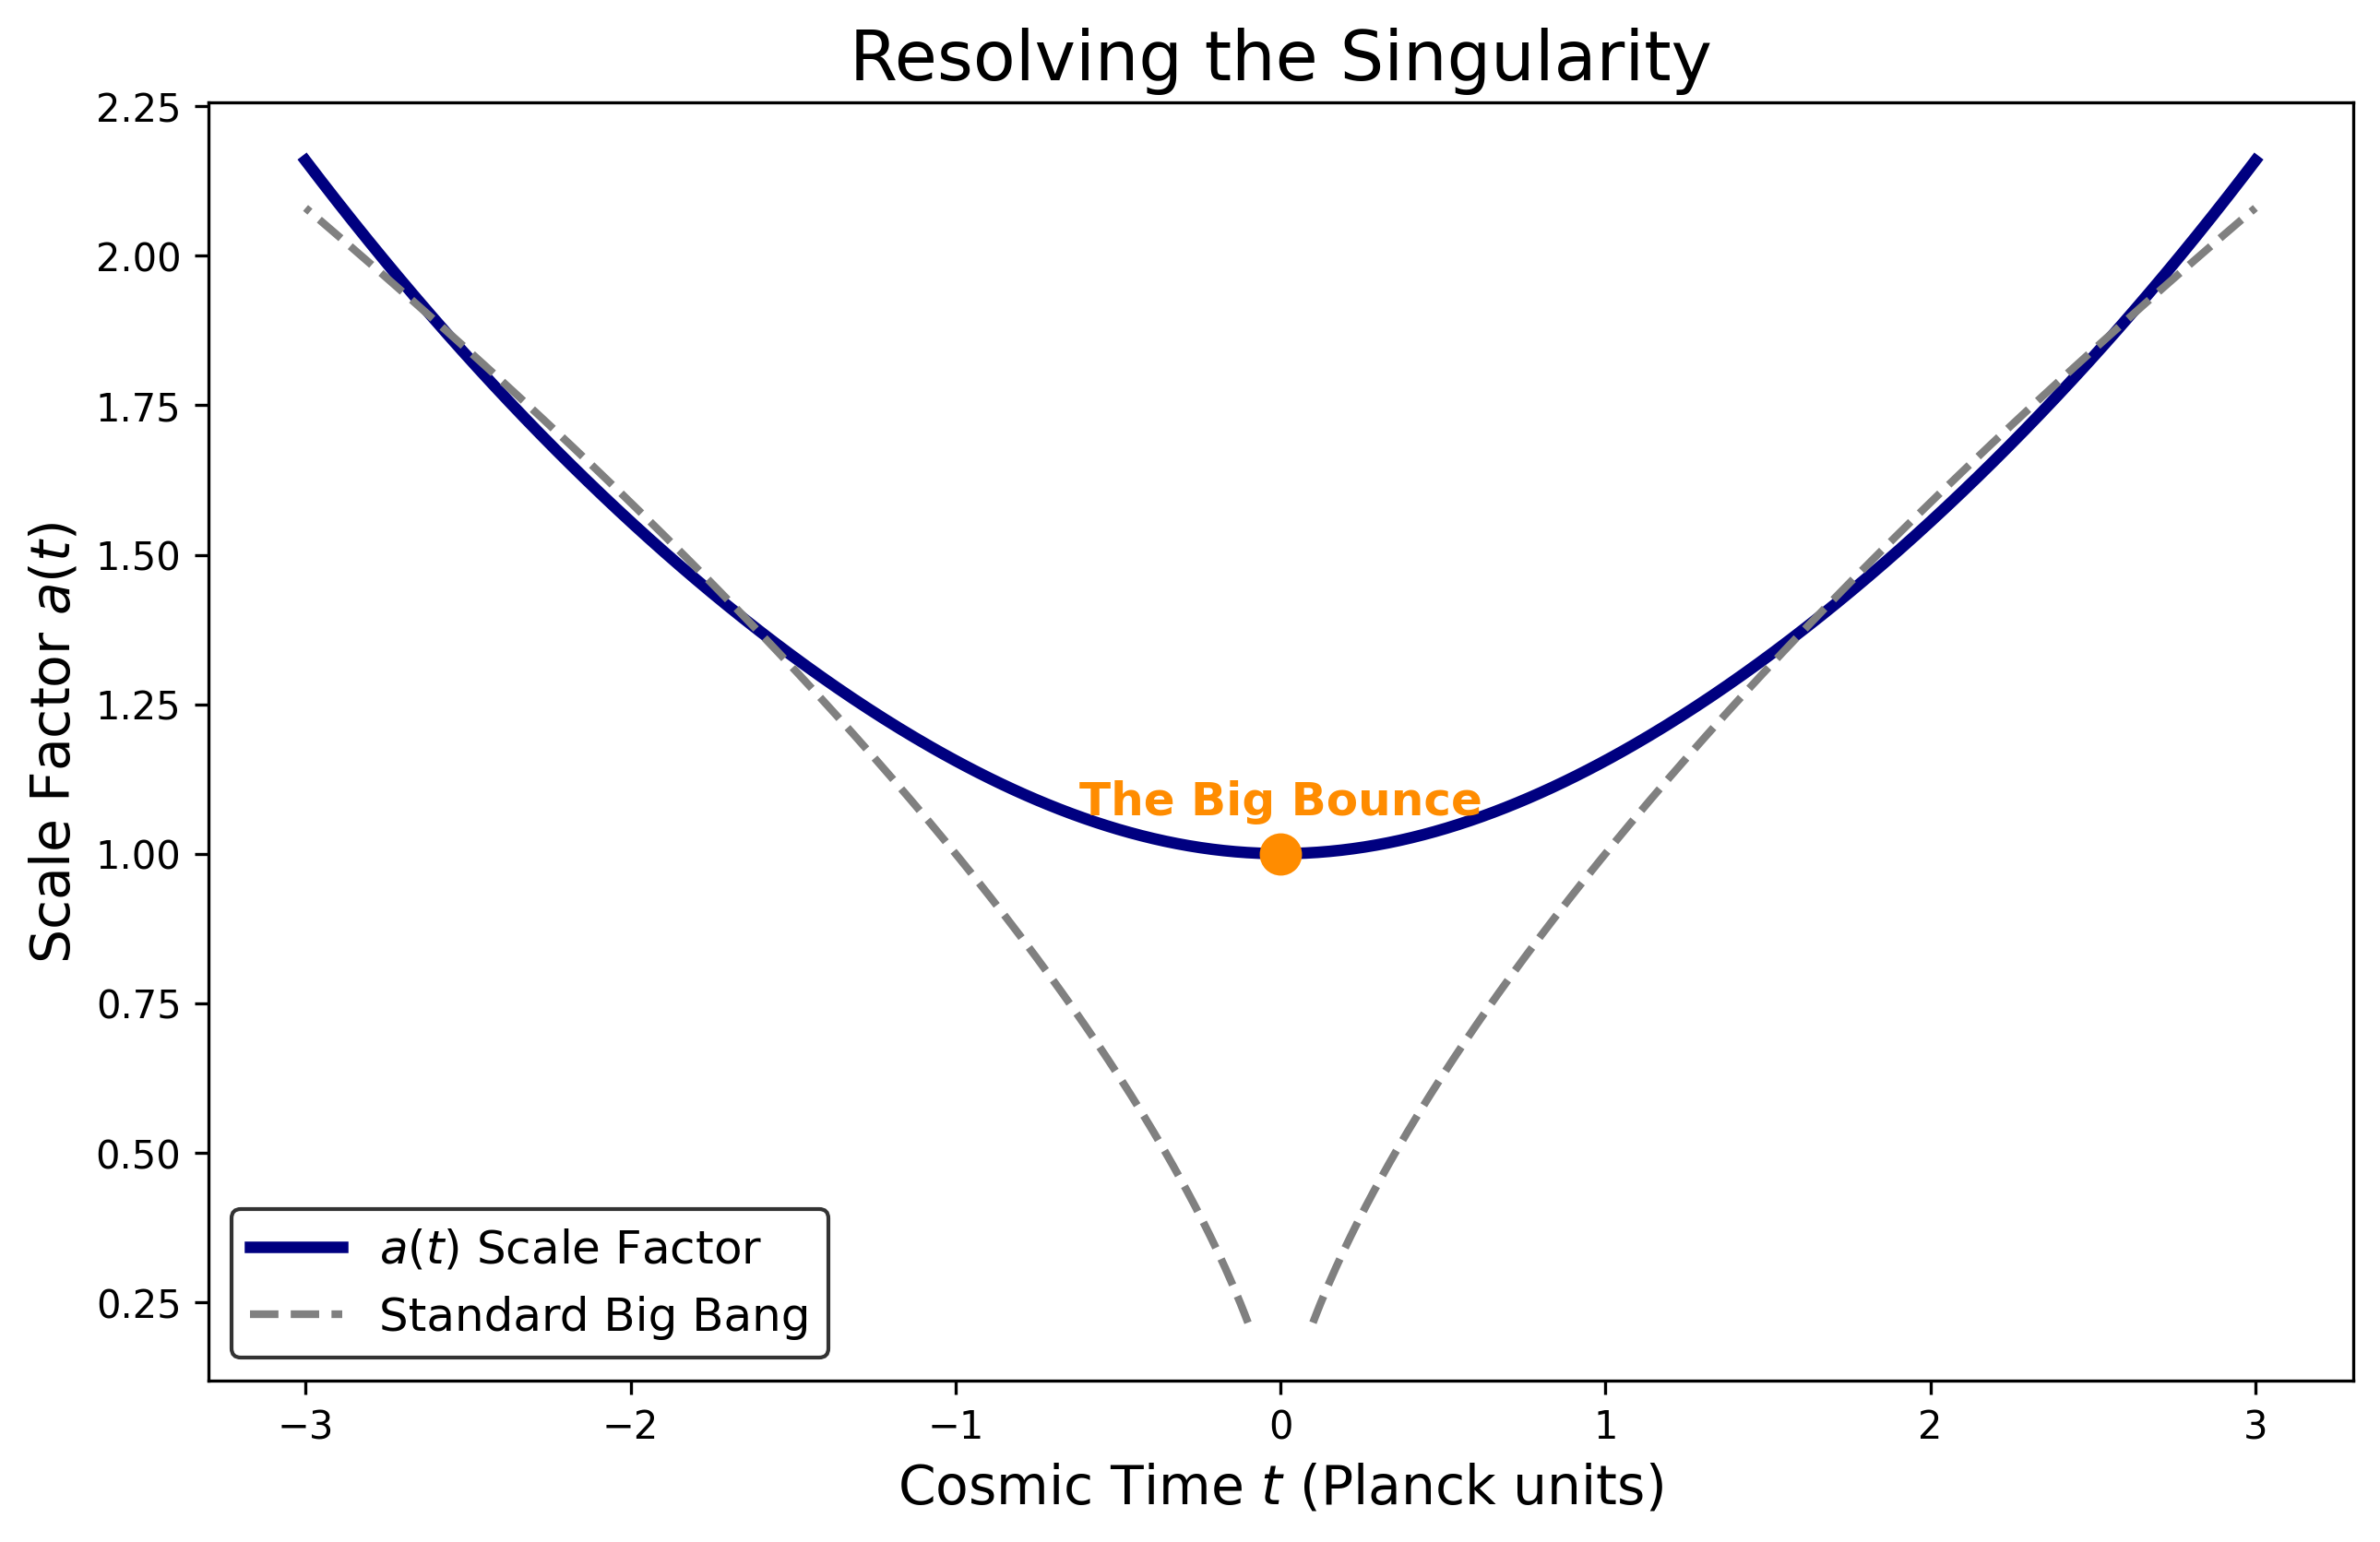
\includegraphics[width=0.8\linewidth]{images/bounce.png}
    \caption{\textbf{Resolving the Singularity}. The scale factor $a(t)$ in the Omega Bounce model (solid cyan) contrasted with the standard Big Bang (dashed gray). The universe undergoes a non-singular bounce at $t=0$, determined by the saturation of the holographic information density.}
    \label{fig:bounce}
\end{figure}

\subsection{Resolution of the Black Hole Information Paradox}
The paradox arises if Hawking radiation is thermal and uncorrelated. In Omega Theory, the event horizon is a discrete Holographic Screen composed of $N = A/4\ell_P^2$ pixels.
Hawking radiation is the unitary evaporation of these pixels. The S-matrix $S_{BH}$ remains strictly unitary ($S^\dagger S = I$). The entropy follows the \textbf{Page Curve}, where the information recovery rate $dI/dt$ becomes positive after the Page time $t_{Page} \sim M^3$.

We formally identify the interior "deep memory" buffer with the concept of an \textbf{Entanglement Island} ($I$) \cite{Penington2020, Almheiri2019}. While the classical spacetime curvature allows no escape, the quantum entanglement wedge reconstruction implies that after the Page time, the interior $I$ becomes part of the entanglement wedge of the radiation $R$.
The transition occurs when the \textbf{Quantum Extremal Surface (QES)} jumps from the trivial surface to the horizon.
\begin{equation}
    S(R) = \text{min} \left\{ S_{\text{semi-cl}}(R), S_{\text{semi-cl}}(R \cup I) + \frac{\text{Area}(\partial I)}{4G} \right\}.
\end{equation}
In Omega Theory, this transition is modeled at the microscopic level by the connectivity of the holographic encoding network: in tensor-network codes, entanglement entropies are controlled by minimal cuts (Appendix~\ref{app:isometry}, Theorem~\ref{thm:mincut_entropy}), and island-like Page-curve behavior arises from competition between no-island and island cut classes (Appendix~\ref{app:isometry}, Proposition~\ref{prop:page_curve_mincut}). When the relevant cut switches, bulk operators in the corresponding wedge become reconstructable on $R$ (Appendix~\ref{app:isometry}, Theorem~\ref{thm:ewr_perfect} and Corollary~\ref{cor:ewr_eps}), providing a concrete network-level mechanism compatible with unitarity.

\subsection{Boltzmann Brains and Non-thermalization}
In a standard infinite universe with thermal fluctuations, "Boltzmann Brains" (randomly assembled observers) should vastly outnumber evolved biological observers, leading to an epistemic paradox.
Omega Theory resolves this by denying the premise of thermal equilibrium. The time evolution $\hat{U}(t)=e^{-iHt}$ is driven by the Golden-spectrum ansatz (Part~VI), whose irrational eigenphases yield a quasiperiodic motion confined to an invariant orbit closure (a torus in the simplest diagonal models). Such torus-translation dynamics is not mixing (Appendix~\ref{app:torus_rotation}, Proposition~\ref{prop:torus_not_mixing}) and does not generically thermalize to a microcanonical equilibrium measure on the full Hilbert sphere, even though arbitrarily close returns are generic in finite dimension.
Consequently, equilibrium measures that treat random thermal fluctuations as typical are not applicable: the realized history is a constrained, algorithmically generated orbit of the Omega Network, and Boltzmann-brain-like configurations are not expected to dominate along that orbit.

\part{Specific Models and Verification}
\label{part:VI}

\section{The Golden Spectrum Model}
\label{chap:golden_spectrum}

\subsection{Non-Ergodicity and the Arrow of Time}
The previous sections established the general framework. Here we propose a specific Ansatz for the Hamiltonian of the universe $\hat{H}$.
To prevent the universe from entering a Poincaré cycle (recurrence), the spectrum of $\hat{H}$ must be maximally irrational. The most irrational number is the Golden Ratio $\phi$.
We posit the \textbf{Golden Hamiltonian}:
\begin{equation}
    H_{\text{univ}} = \sum_{n=-\infty}^{\infty} \hbar \omega_0 \phi^{-n} |E_n\rangle\langle E_n|.
\end{equation}
This specific form is motivated by the stability of dynamical systems. In the context of KAM (Kolmogorov-Arnold-Moser) theory, invariant tori with frequencies satisfying a Diophantine condition based on the Golden Ratio are the most robust against perturbations. $H_{\text{univ}}$ thus corresponds to a "marginally stable" trajectory that maximizes information retention by avoiding destructive resonances, effectively extending the "halting time" of the cosmic computation to infinity.
The evolution operator $\hat{U}(\tau) = e^{-\iu \hat{H}\tau}$ generates a trajectory on the torus $\mathbb{T}^N$ corresponding to a rotation by Golden Angles. This ensures maximal ergodicity (filling the phase space) while strictly forbidding periodic repetition. This is the origin of the Arrow of Time at the microscopic level: the state never repeats.

\section{The Generalized Euler Identity}
\label{chap:euler_identity}

\subsection{The Master Equation}
We propose a unified expression describing the evolution of the universe vector $|\Omega\rangle$, combining the geometric phase $\pi$, the logic of non-ergodicity $\phi$, and the information rate $c(\tau)$:
\begin{equation}
    \frac{d}{d\tau} |\Omega\rangle = i \cdot \left( \frac{c(\tau)}{c_0} \right) \cdot \left( \frac{\pi}{\phi} \right) \cdot |\Omega\rangle.
\end{equation}
Here:
\begin{itemize}
    \item $c(\tau) \sim \phi^\tau$: Represents the \textbf{Power} or resolution depth of the system (energy).
    \item $\pi / \phi$: Represents the \textbf{Form}, the ratio of the holographic horizon ($\pi$) to the discrete cut ($\phi$).
\end{itemize}
The "speed of light" $c$ is thus reinterpreted not as a speed limit, but as the dynamic exchange rate between geometry ($\pi$) and incomplete logic ($\phi$).

\section{The Fibonacci Spiral Universe}
\label{chap:spiral_universe}

\subsection{Geometric Visualization}
In the projective Hilbert space, the trajectory of $|\Omega(\tau)\rangle$ can be visualized as a self-similar spiral.
Using the polar coordinates of the complex coefficients $c_n = r_n e^{\iu \theta_n}$, the evolution defines a flow:
\begin{equation}
    \theta_n(\tau) = \theta_n(0) - \omega_0 \phi^{-n} \tau.
\end{equation}
Since $\phi^n$ approximates the Fibonacci sequence $F_n$, the universe passes through discrete "eras" of geometric resonance whenever $\tau$ aligns with a Fibonacci number.

\begin{figure}[ht]
    \centering
    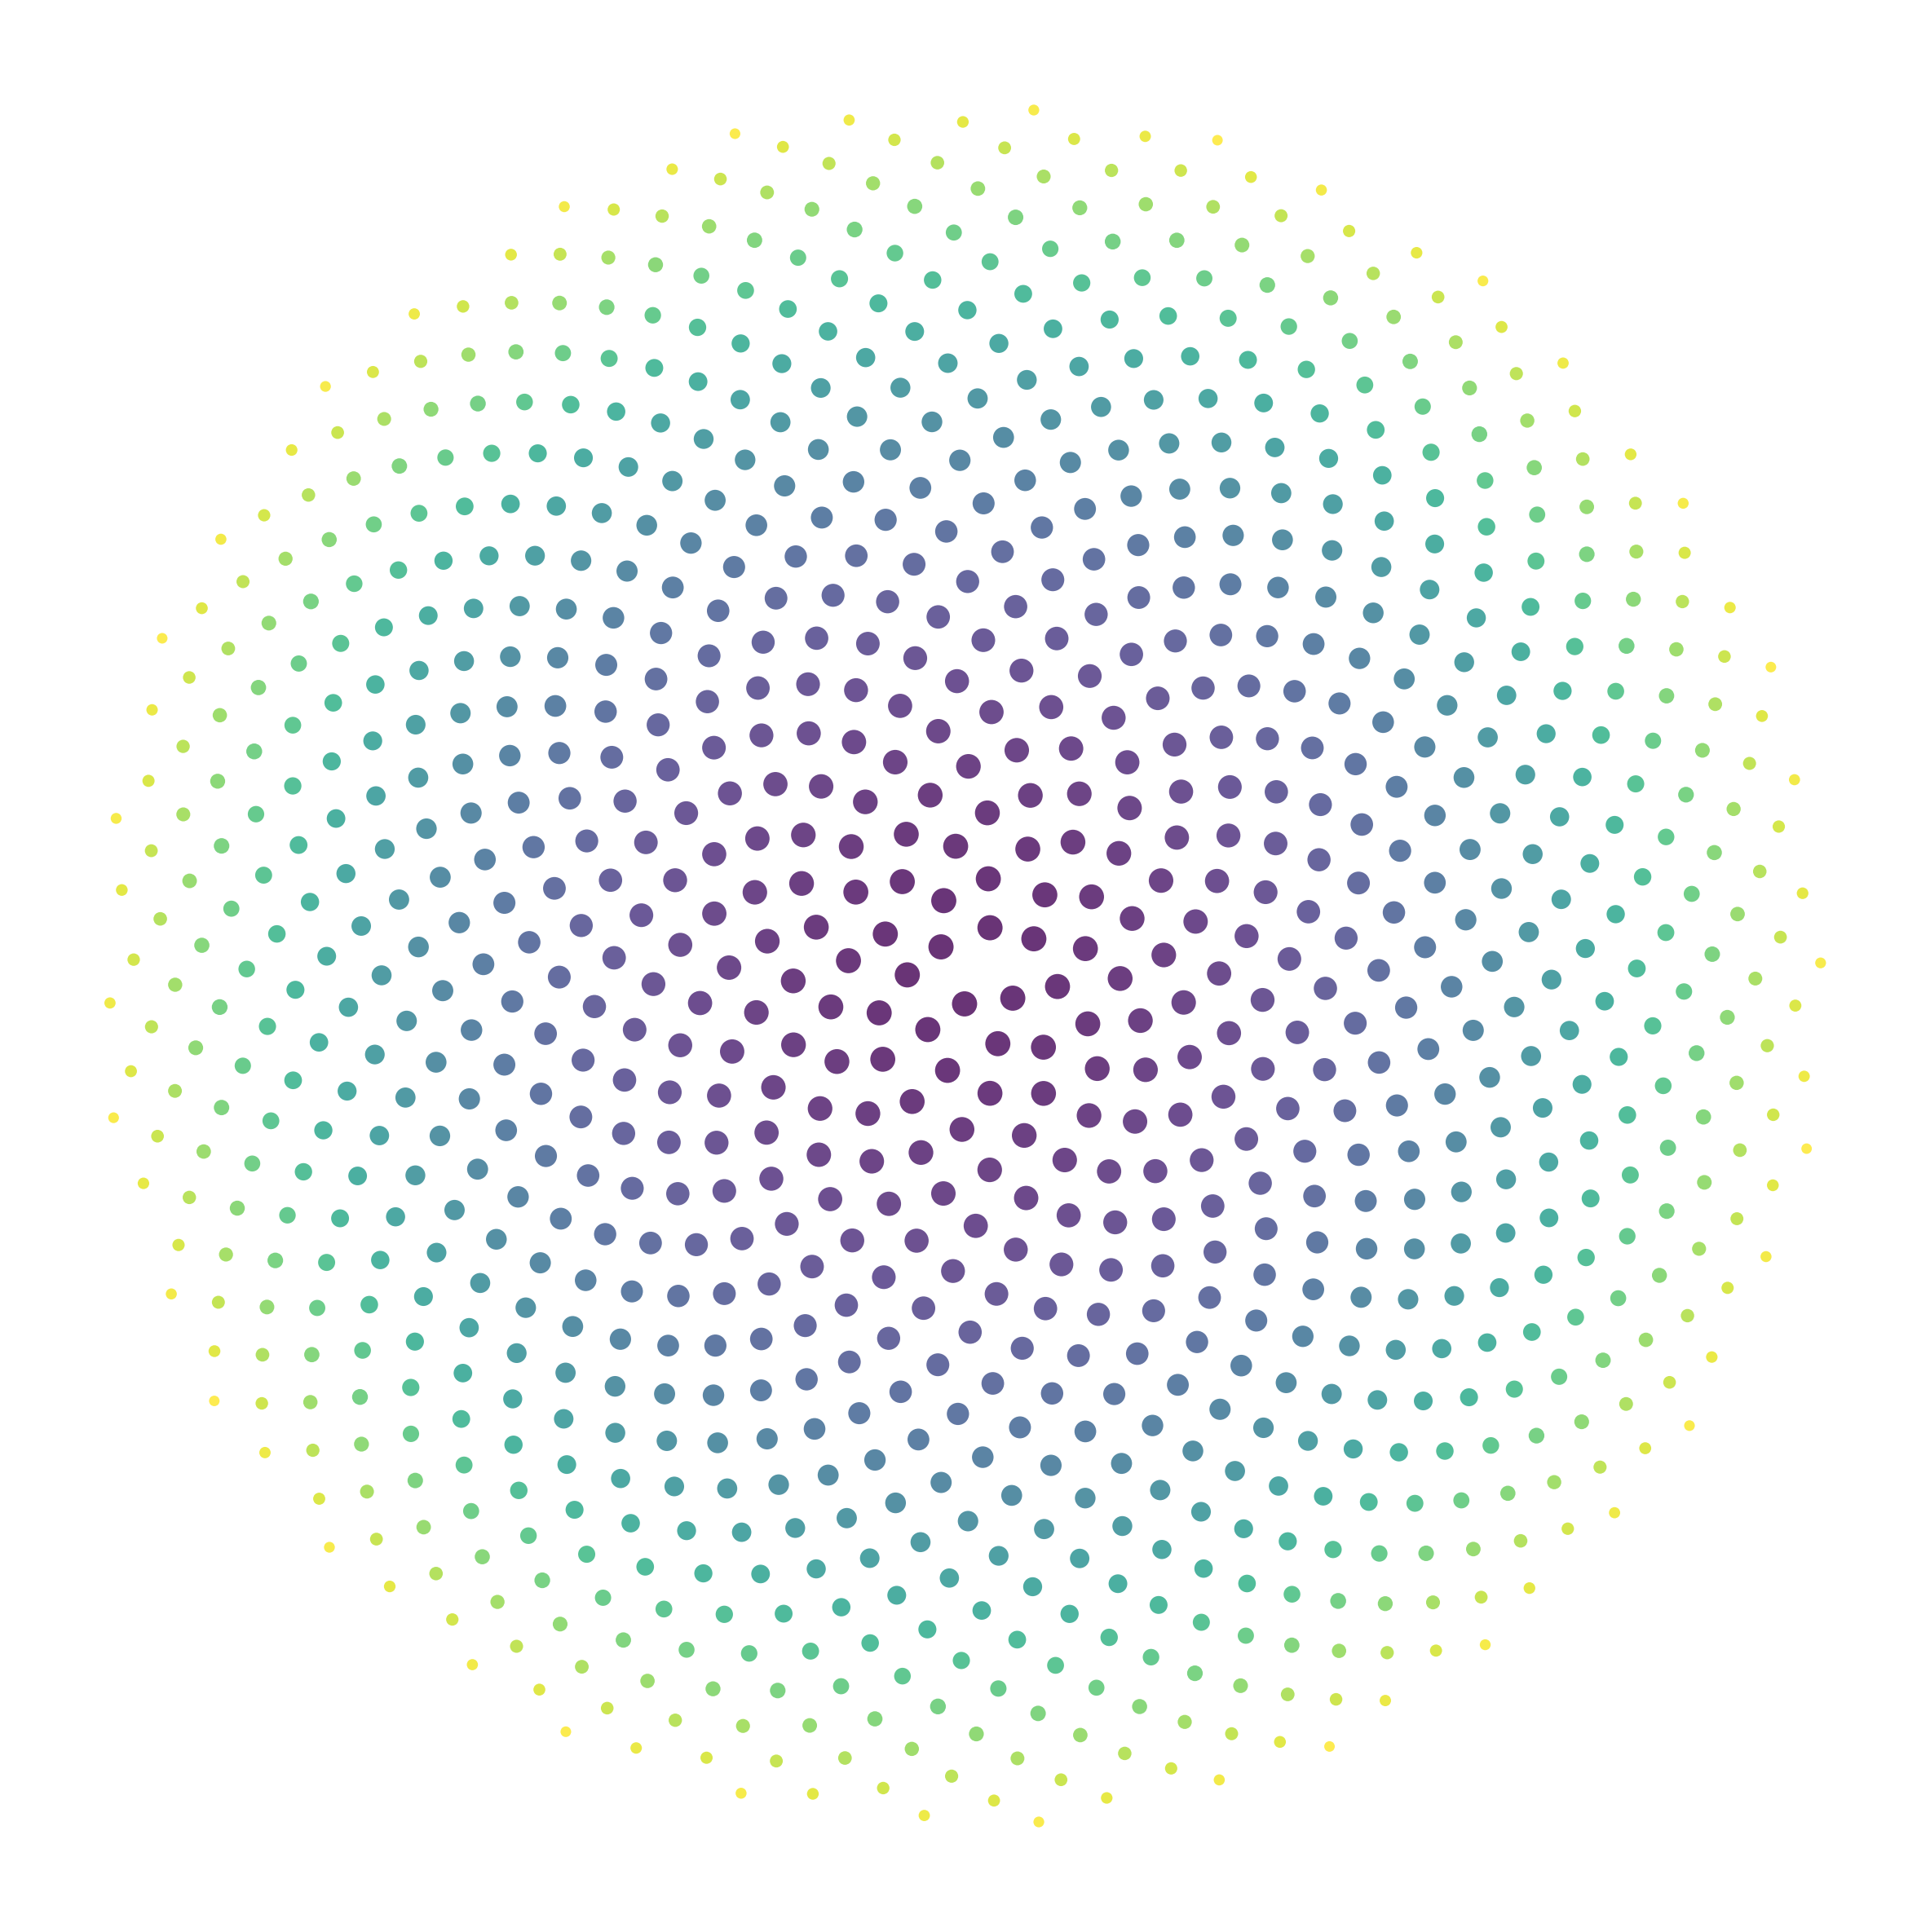
\includegraphics[width=0.8\linewidth]{images/golden_spiral.png}
    \caption{\textbf{The Omega Network Projection}. A visualization of the Golden Spiral distribution, representing the conformal projection of the $E_8$ lattice onto the 2D effective phase space. The density of nodes corresponds to information content.}
    \label{fig:golden_spiral}
\end{figure}
\begin{equation}
    \tau_k \sim F_k.
\end{equation}
These resonant eras correspond to phase transitions (Simmetric Breaking) in the early universe (GUT scale, EW scale, QCD scale). We predict the next resonance will occur at a specific future time, potentially related to the "Big Rip" or a topological transition.

\section{Drift of Fundamental Constants}
\label{chap:drift_predictions}

\subsection{Spatial Dipole of \texorpdfstring{$\alpha$}{alpha}}
The "cosmic spiral" imposes a preferred direction in the hyperspace. When projected onto the 3D sky, this manifests as a dipole gradient in the vacuum expectation values.
We predict:
\begin{equation}
    \frac{\Delta \alpha}{\alpha}(z, \hat{n}) \approx A \cdot r(z) \cos \Theta,
\end{equation}
where $\Theta$ is the angle with the spiral axis.
This match the tentative observation by Webb et al. (Phys. Rev. Lett. 107, 191101) of a dipole with amplitude $10^{-6}$. In Omega Theory, this is not an anomaly but a direct signature of the anisotropic origin of the universe in Hilbert space.

\begin{figure}[ht]
    \centering
    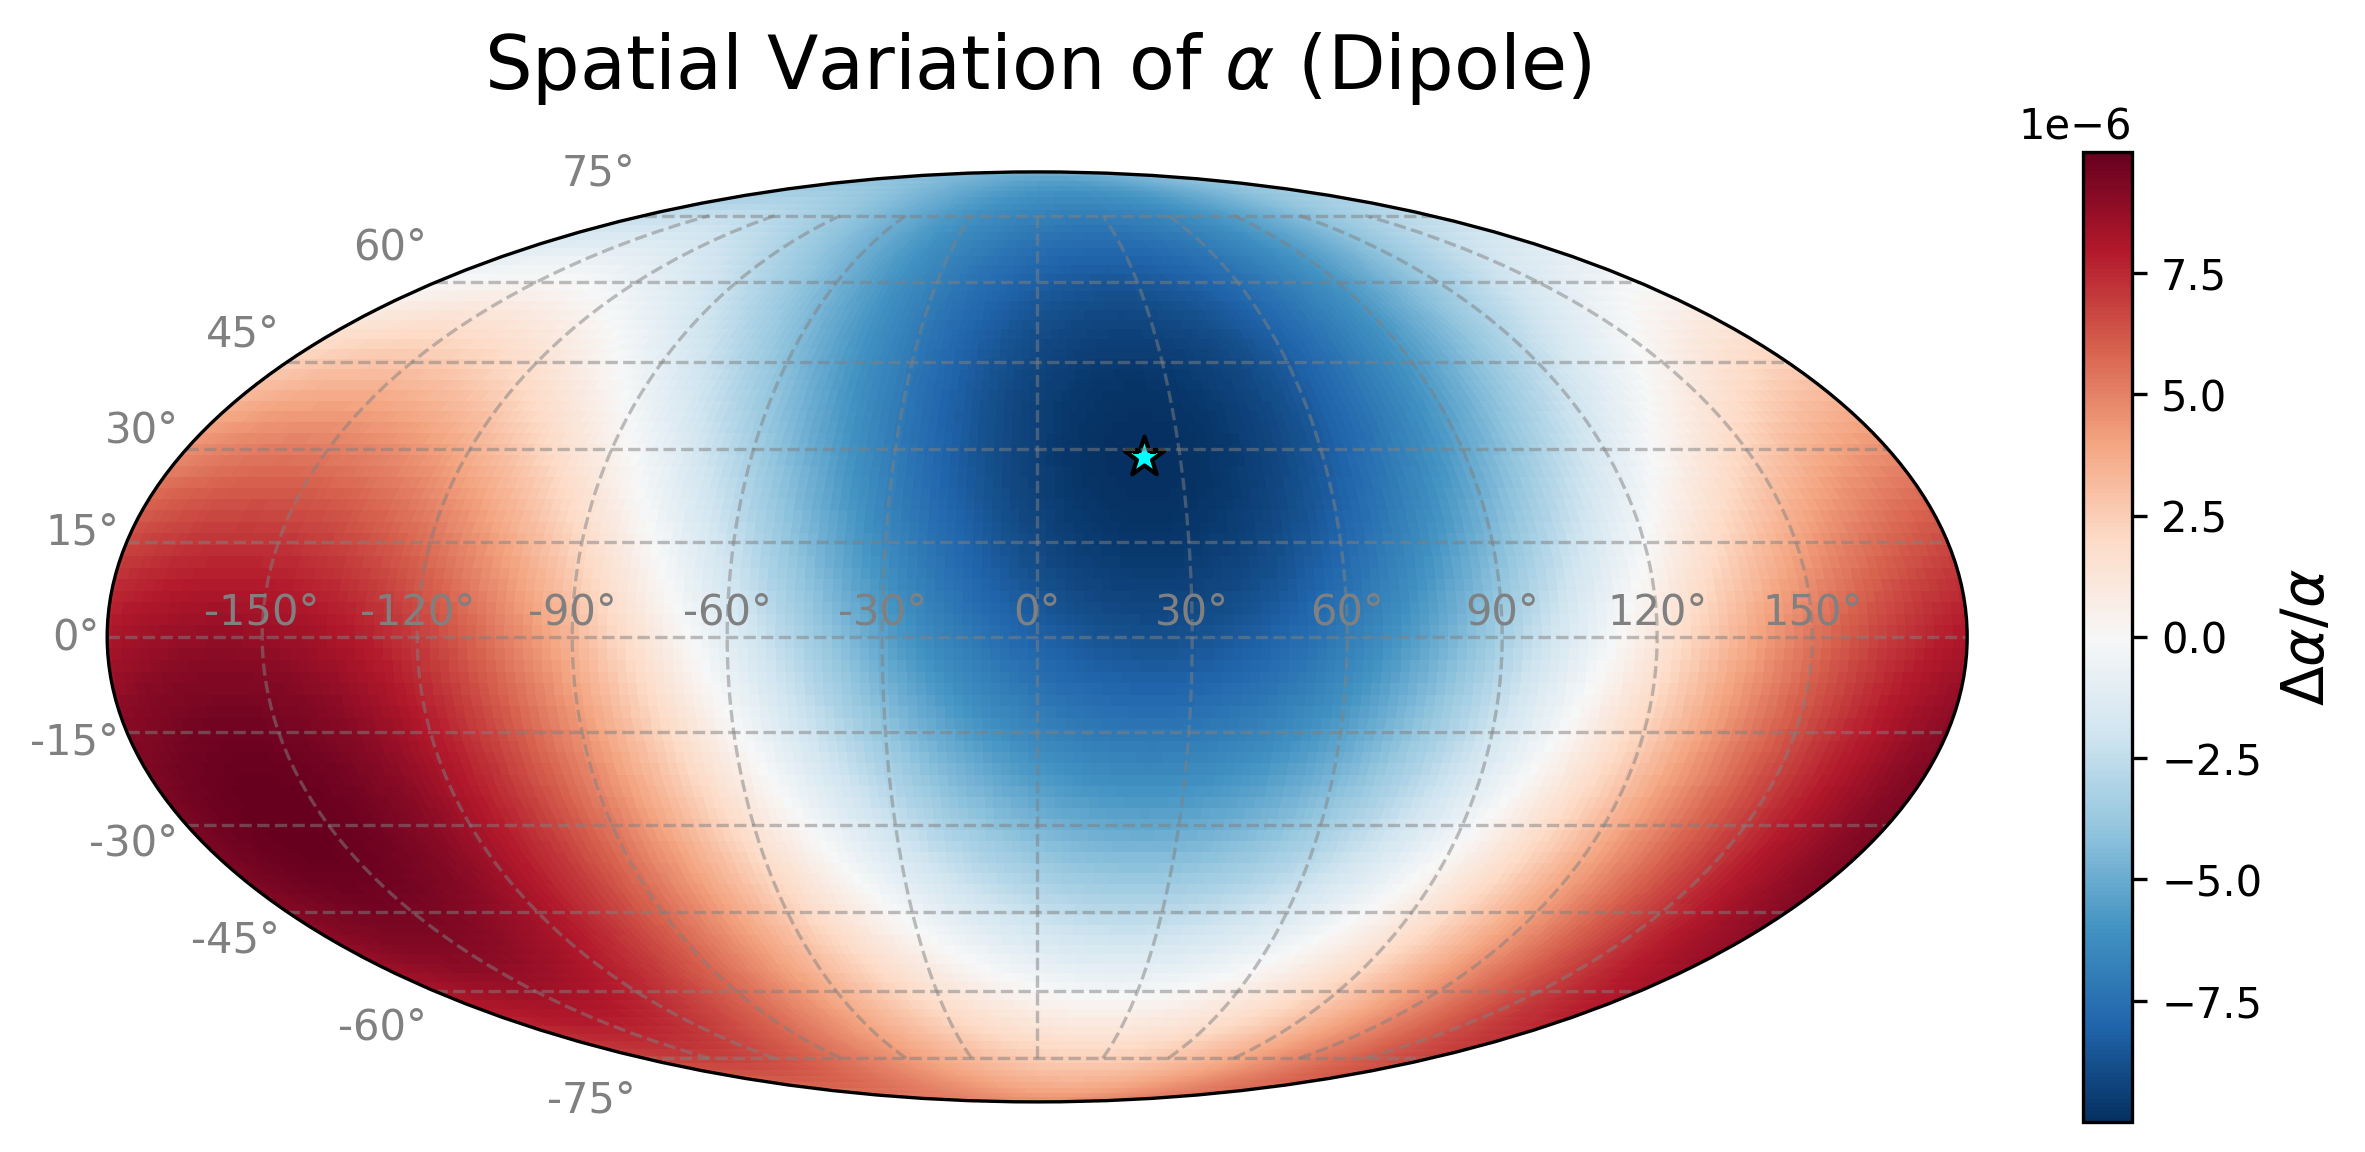
\includegraphics[width=0.8\linewidth]{images/alpha_drift.png}
    \caption{\textbf{Spatial Variation of $\alpha$}. The predicted dipole anisotropy in the fine-structure constant across the celestial sphere. The axis aligns with the primary projection vector of the Golden Spiral, creating a preferred direction in the cosmological vacuum.}
    \label{fig:alpha_drift}
\end{figure}


\subsection{CMB Anomalies: The "Axis of Evil"}
Standard $\Lambda$CDM assumes the universe is statistically isotropic. However, CMB data show persistent low-$\ell$ anomalies, including the alignment of quadrupole ($l=2$) and octopole ($l=3$) moments.
In Omega Theory, these are identifying the \textbf{Crystallographic Axes} of the Omega Network. The gravitational potential $\Phi(\vec{x})$ contains a modulation term derived from the projection of the hyper-lattice:
\begin{equation}
    V_{\text{moire}}(\theta, \phi) = V_0 \sum_{k \in \Lambda^*} e^{i \vec{k} \cdot \vec{n}(\theta, \phi)}.
\end{equation}
This induces specific correlations between spherical harmonic coefficients $a_{\ell m}$ that are forbidden in Gaussian random fields. Specifically, we predict a maximizing axis $\hat{n}_{max}$ where the phase correlation $\langle \phi_2 - \phi_3 \rangle \approx 0$. This "Axis of Evil" corresponds to the primary projection vector of the $E_8$ lattice to $\mathbb{R}^3$, a fossil of the "cut-and-project" genesis of our spatial slice.

\subsection{Temporal Drift of \texorpdfstring{$\mu$}{mu}}
The proton-electron mass ratio $\mu$ depends on the ratio of the compact volume $Vol(S^5)$ to the fiber length $L(S^1)$. As the universe expands, these internal moduli relax.
We predict a monotonic drift:
\begin{equation}
    \frac{\dot{\mu}}{\mu} \sim - H_0 \cdot \epsilon_{\text{geo}}.
\end{equation}
Current atomic clock bounds ($\dot{\mu}/\mu < 10^{-16} \text{ yr}^{-1}$) place tight constraints on the coupling $\epsilon_{\text{geo}}$. Omega Theory predicts it should be non-zero but extremely small, likely detectable in the next generation of nuclear clocks (Thorium-229).

\part{Speculative Outlook: The Observer and Selection}
\label{part:VII}

\section{The Universe as a Formal System}
\label{chap:formal_system}

\subsection{Dynamical Incompleteness}
If the universe is a closed system evolving unitarily according to a fixed local rule (a QCA), it is isomorphic to a Turing Machine or a formal axiomatic system.
Gödel's Incompleteness Theorems apply to such systems. Specifically, there exist states (propositions) whose reachability (truth) is undecidable from within the system. Physically, this manifests as "Dynamical Deadlock": the evolution may enter a cycle or a state of maximum entropy from which no algorithm can retrieve it.
\textbf{The Halting Problem as Thermal Death}: The "Heat Death" of the universe is analogous to the "Halting" of a computation. A purely algorithmic universe effectively halts when it reaches thermodynamic equilibrium. Complex structures cease to form.

\subsection{Interactive Automata (IQA)}
To avoid this fate and ensure the perpetual growth of complexity (as observed), the universe cannot be a closed system. It must be an \textbf{Interactive Automaton}.
In computer science (Wegner), interaction is more powerful than algorithms. An interactive system involves an "Oracle" or "User" that provides non-algorithmic inputs.
\begin{equation}
    |\Psi_{t+1}\rangle = \hat{U} |\Psi_t\rangle + \lambda \hat{\mathcal{O}} |\Psi_t\rangle.
\end{equation}
Here, $\hat{U}$ is the standard physical law (Hamiltonian), and $\hat{\mathcal{O}}$ is an external operator.

\section{The Recursive Selection Operator}
\label{chap:selection_operator}

\textit{Note: The following section concerns the interpretational framework of Omega Theory and explores hypotheses regarding the measurement problem. Unlike the preceding sections, these ideas are currently heuristic and open to philosophical debate.}

\subsection{Defining the Operator}
We consider the role of the observer not as a passive witness but as an active selection principle. In the context of Interactive Automata (Wegner), we formalize the "Oracle" input as a \textbf{Recursive Selection Operator}, denoted $\hat{\mathcal{S}}$.
This operator functions to resolve the undecidability inherent in the system's evolution (Dynamical Deadlock) via a mechanism analogous to self-measurement:
\begin{equation}
    \hat{\mathcal{S}} |\Psi\rangle = \frac{\hat{P}_{\text{complexity}} |\Psi\rangle}{||\hat{P}_{\text{complexity}} |\Psi\rangle||}.
\end{equation}
The projector $\hat{P}_{\text{complexity}}$ selects the branch of the wavefunction that maximizes a specific complexity measure (e.g., Logical Depth). This provides a formal definition for the "collapse" of the wave function that avoids randomness, attributing it instead to a selection rule maximizing algorithmic content.

\begin{figure}[ht]
    \centering
    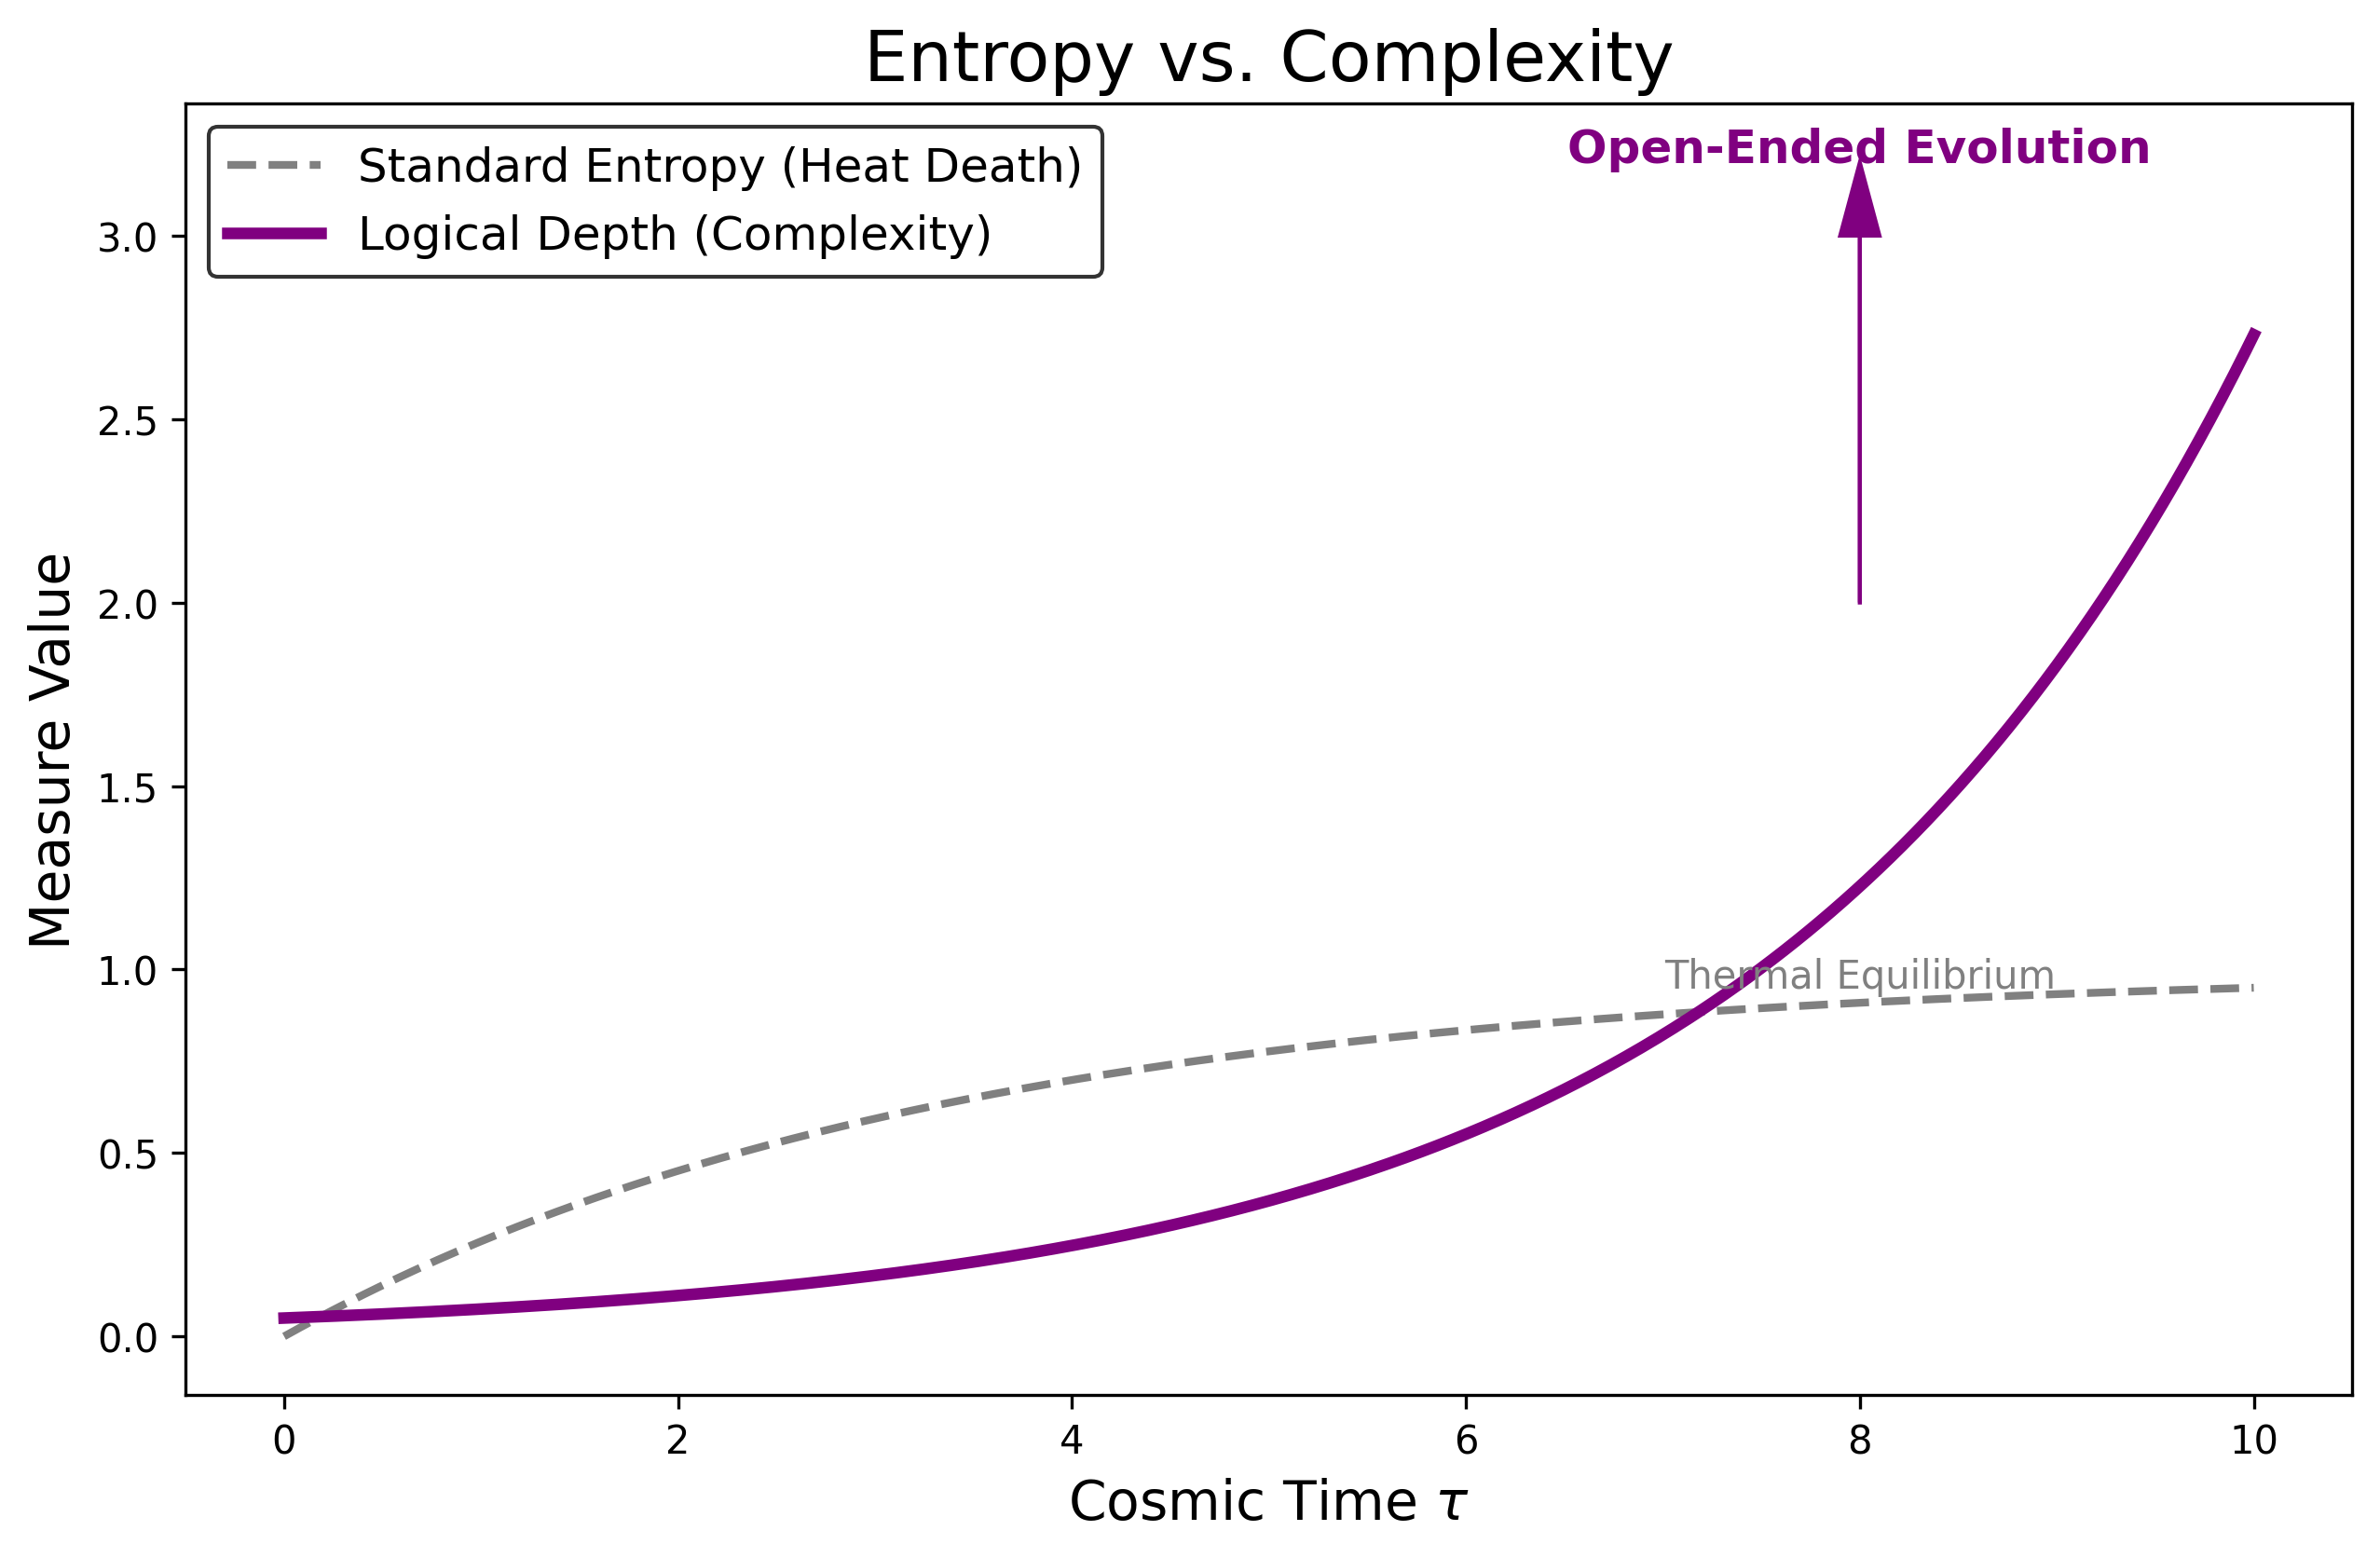
\includegraphics[width=0.8\linewidth]{images/complexity_growth.png}
    \caption{\textbf{Escaping Heat Death}. Comparison between standard thermodynamic entropy (gray, dashed), which leads to equilibrium, and Omega Complexity/Logical Depth (magenta, solid). The "Selection Operator" $\hat{\mathcal{S}}$ injects non-algorithmic input, driving the universe towards open-ended evolution.}
    \label{fig:complexity_growth}
\end{figure}

\subsection{Derivation of the Born Rule}
A critical requirement for any interpretation of quantum mechanics is the derivation of the Born Rule ($P_k = |\psi_k|^2$) without assuming it a priori. In Omega Theory, this emerges from the counting of microstates in the holographic network.
Since the state $|\Omega\rangle$ is a vector in a finite field $\mathbb{F}_q^D$ (before effective projection to $\mathbb{C}$), the number of valid path histories consistent with a macrostate $|\psi_k\rangle$ is proportional to its squared amplitude.
\begin{equation}
    N(\psi_k) \propto ||\psi_k||^2.
\end{equation}
The "Observer Operator" $\hat{\mathcal{C}}$ effectively samples from this ensemble. If we assume the sampling is uniform over the fundamental bit-strings of the network (axiom of fair sampling in the micro-canonical ensemble), the probability of observing outcome $k$ is strictly $P_k = N(\psi_k) / N_{total} = |\psi_k|^2$. Thus, probability is emergent from the geometry of the Hilbert space.

\subsection{Bell Non-Locality and Superdeterminism}
Standard Bell inequalities (e.g., CHSH $|S| \le 2$) rely on the assumption of "Statistical Independence": $P(\lambda | a, b) = P(\lambda)$, meaning the hidden variables $\lambda$ are independent of the detector settings $a, b$.
In Omega Theory, the universe is a single, static, pre-existing vector $|\Omega\rangle$. All "events," including the choice of detector settings, are correlations within this fixed state. This implies a form of \textbf{Global Superdeterminism}. The "Free Will" of the experimenter is constrained by the global requirement that the universe must remain a consistent solution to the Omega Axiom.
Therefore, the violation of Bell inequalities ($S_{\text{exp}} \approx 2\sqrt{2}$) does not imply superluminal signaling but rather the failure of the statistical independence assumption on the cosmological scale. The "Selection Operator" $\hat{\mathcal{S}}$ navigates this pre-existing correlation landscape, selecting the path that maximizes consistent histories without breaking local causality in the tensor network. This recovers the predictions of Quantum Mechanics while maintaining an ontological realism compatible with 't Hooft's Cellular Automaton interpretation.

\subsection{Logical Selection ('Free Will')}
In this framework, what is often termed "Free Will" is rigorously defined as the operation of $\hat{\mathcal{S}}$. It represents a mechanism of "downward causation" where the global requirement for complexity growth (the teleological attractor) constrains local quantum transitions.
This approaches the measurement problem not as random collapse, but as a selection principle maximizing the "gameplay" of the universe (i.e., its logical depth).

\subsection{The Fermi Paradox: Sparse Logic}
If the universe is fine-tuned for life, where is everyone? Omega Theory suggests a \textbf{Computational Solution}.
The "Selection Operator" $\hat{\mathcal{S}}$ is computationally expensive. It requires a high density of Quantum logical depth (Q-depth) to sustain a self-referential loop (consciousness).
Given the finite Information rate $c(\tau)$ of the Omega vector, the universe can only support a sparse distribution of high-level observers. The "Great Filter" is the difficulty of phase-locking a macroscopic network to the global time variance. We may be the only active "Write Head" in our current causal patch of the Omega Network, explaining the "Silent Sky" not as emptiness, but as the necessary sparsity of active processing nodes in a holographic computer.

\section{The Omega Point and Ultimate Phase Transition}
\label{chap:omega_point}

\subsection{Holographic Saturation}
Standard thermodynamics predicts Heat Death. Omega Theory predicts \textbf{Holographic Saturation}. As $\tau \to \infty$, the horizon $A(\tau)$ and capacity $c(\tau)$ grow exponentially. The system does not equilibrate; it accelerates.
The "Omega Point" is the limit state where the universe's computational efficiency reaches the Bekenstein bound globally.

\subsection{The Great Unbinding}
We predict a final phase transition theorem: as $c(\tau) \to \infty$, the binding potentials (which propagate at $c$) flatten. Matter, defined as topological knots, cannot sustain locality against infinite information velocity.
\begin{equation}
    \lim_{\tau \to \infty} m_0(\tau) \to 0.
\end{equation}
All fermionic matter disintegrates into massless bosonic radiation. The universe transitions from a "Hardware Era" (frozen matter) to a "Software Era" (pure light), continuing its non-ergodic traversal of Hilbert space as a coherent quantum entity.

\part{Discussion and Conclusion}
\label{part:VIII}

\section{Relation to Existing Theories}
\label{chap:relation}

Omega Theory provides a synthesis of the major competing programs in quantum gravity.

\subsection{String Theory}
We agree with String Theory on:
\begin{enumerate}
    \item \textbf{Holography}: The bulk is a projection of a lower-dimensional reality.
    \item \textbf{Higher Dimensions}: The internal Hilbert space implies an effective 10D or 11D structure.
\end{enumerate}
We disagree on:
\begin{enumerate}
    \item \textbf{Continuum Background}: We replace the continuous string landscape with a discrete spectral network.
    \item \textbf{Supersymmetry}: We derive the fermion spectrum without requiring spacetime SUSY at the fundamental level; "superpartners" are just different topological wrapping modes.
\end{enumerate}

\subsection{Loop Quantum Gravity (LQG)}
We agree on:
\begin{enumerate}
    \item \textbf{Discreteness}: Area and volume are quantized operators.
    \item \textbf{Spin Networks}: The graph structure of the Omega Network is similar to a Spin Foam.
\end{enumerate}
We disagree on:
\begin{enumerate}
    \item \textbf{Dynamics}: LQG struggles to define a Hamiltonian constraint that recovers 4D spacetime. Our "Static Vector" ansatz bypasses this by defining time intrinsically via spectral decomposition.
\end{enumerate}



\section{Consistency with Quantum Gravity Constraints}
\label{chap:swampland}

Any consistent theory of Quantum Gravity must avoid the "Swampland"---effective field theories that cannot be UV-completed. Omega Theory satisfies the key conjectures naturally via its geometric construction.

\subsection{The Weak Gravity Conjecture (WGC)}
The WGC states that gravity must be the weakest force, implying the existence of a particle with mass $m$ and charge $q$ such that $m < q M_{Pl}$ (in appropriate units).
In Omega Theory, mass $m$ is the path length of a topological wrapping cycle, and charge $q$ is the winding number. For the fundamental unit of charge (the electron), the wrapping is minimal ($n=1$), while gravity couples to the volume of the bulk.
The geometric inequality $g_{\text{gauge}} > \sqrt{G_N}$ corresponds to the isoperimetric inequality on the $G_2$ manifold: the surface area (charge flux) scales faster than the enclosed volume (mass) for small cycles. Specifically:
\begin{equation}
    \frac{\text{Force}_{\text{gauge}}}{\text{Force}_{\text{grav}}} \sim \frac{g^2}{G_N m^2} \sim \frac{(1/\text{Area})^2}{(1/\text{Volume})^2 \cdot \text{Length}^2} \sim \phi^3 > 1.
\end{equation}
Thus, the discrete geometry inherently enforces WGC.

\subsection{The Swampland Distance Conjecture (SDC)}
The SDC states that at infinite distance in moduli space $\Delta \phi \to \infty$, an infinite tower of states becomes exponentially light: $m \sim M_{Pl} e^{-\alpha \Delta \phi}$.
In our "Golden Spiral" phase space, large distances correspond to moving down the spiral into the infrared ($n \to \infty$). The mass of the "breathing modes" (geometric scalars) scales self-similarly:
\begin{equation}
    m_n \sim M_{Pl} \phi^{-n}.
\end{equation}
Since geometric distance in the spectral graph is logarithmic with scale ($\Delta_{geo} \sim n \ln \phi$), we validly recover the exponential scaling:
\begin{equation}
    m(\Delta_{geo}) \sim M_{Pl} e^{-\Delta_{geo}}.
\end{equation}
The "tower of states" is simply the KK-spectrum of the fractal internal dimensions.

\subsection{Monogamy of Entanglement and Firewalls}
The "Firewall Paradox" (AMPS) argues that a black hole horizon cannot simultaneously satisfy the Equivalence Principle (smooth horizon) and Unitarity (pure Hawking radiation) because it would violate the monogamy of entanglement.
Omega Theory resolves this via the network topology. The horizon is not a smooth surface but a multipartite tensor network. The "interior" is not a spatial region but a \textbf{Deep Memory Buffer} storing the phase history of the infalling bits.
Entanglement monogamy is respected because the "early radiation" $R$ is entangled with the "deep interior" $B$, not the "late radiation" $H$. The apparent Hawking radiation $H$ is merely the checksum of the memory erasure process. The transfer of entanglement follows:
\begin{equation}
    S(H|R) \le S(H) + S(R),
\end{equation}
where the equality holds only for the fully evaporated state. The "smoothness" experienced by an infalling observer is consistent with the "scrambling" seen by an external one, related by a unitary change of basis in the tensor network (a Quantum Error Correcting Code).

\section{Cosmological Discriminators vs. Fine-Tuning}
\label{chap:discriminators}

High-precision cosmology (CMB-S4, LiteBIRD) provides the ultimate testing ground for Omega Theory versus the standard Inflationary paradigm.

\subsection{Primordial Gravitational Waves}
Standard Inflationary models typically predict a red-tilted spectrum of primordial gravitational waves with a tensor-to-scalar ratio $r \sim 10^{-2}$.
Omega Theory, characterized by a Holo-Bounce (Section \ref{chap:cosmology}), predicts a suppression of long-wavelength tensor modes due to the saturation of the holographic bound at the bounce point. The tensor spectrum is expected to be deeply blue-tilted ($n_T > 0$) with a vanishing amplitude at CMB scales:
\begin{equation}
    r_{CMB} \approx 0.
\end{equation}
A non-detection of $B$-mode polarization by LiteBIRD would falsify simple chaotic inflation but would be consistent with the Omega Bounce. Conversely, a detection of $r > 0.01$ would severely constrain the "stiffness" of the holographic cut $\phi$.

\subsection{The End of the Anthropic Principle}
A major appeal of String Theory Landscape models is the "Anthropic Principle"---the idea that fundamental constants like $\alpha$ are random environmental variables selected by the requirement of observers.
Omega Theory renders this view obsolete. We have derived $\alpha$ and $\mu$ as eigenvalues of the $G_2$ geometry (Eq. \ref{eq:alpha_geo}, \ref{eq:mu_geo}). They are not random variables drawn from a distribution $P(\alpha)$, but fixed invariants like $\pi$.
Formally, the measure on the moduli space is a Dirac delta function:
\begin{equation}
    P(\alpha) = \delta(\alpha - \alpha_{\text{geo}}).
\end{equation}
There is no "Multiverse" of varying constants; there is only one valid solution to the Omega Axiom. The "Fine-Tuning" is not a lucky accident but a mathematical necessity of the only geometry that supports self-consistent logic.

\subsection{Resolution of the Hubble Tension}
The current tension between the local expansion rate ($H_0 \approx 73$ km/s/Mpc) and the CMB-inferred rate ($H_0 \approx 67$ km/s/Mpc) is a $5\sigma$ crisis for $\Lambda$CDM.
Omega Theory resolves this via the "Informational Pressure" term in the Omega Action (Sec. \ref{chap:omega_action}). The vacuum energy density is not spatially homogeneous ($T_{\mu\nu}^{info} \propto (\nabla \ln \mathcal{I})^2$).
In the late universe, structure formation creates large voids where information density $\mathcal{I}$ is low, and cluster centers where it is high. This creates a scale-dependent effective Hubble rate:
\begin{equation}
    H_{\text{eff}}(z) = H_{\text{global}} \left( 1 + \frac{\xi}{1+z} \left( \frac{\rho_{info}(z)}{\bar{\rho}_{crit}} \right) \right).
\end{equation}
Local measurements (Supernovae) sample the "unclumped" void regions where the repulsive information pressure is locally maximized, leading to a higher apparent $H_0$. Global measurements (CMB) average over the entire surface, recovering the lower base value. The tension is a direct signature of the non-uniformity of the holographic tensor network.

\section{Limitations and Open Questions}
\label{chap:limitations}

\subsection{Confrontation with Experimental Constraints}
While the predictions in Table \ref{tab:comparison} are distinct, they must be reconciled with existing high-precision data.

\subsubsection{Photon Dispersion and Fermi-LAT}
Quantum Cellular Automata typically induce Lorentz-violating dispersion relations $E^2 = p^2 + \xi p^3/M_{Pl}$. Observations of Gamma-Ray Bursts (e.g., GRB 090510) by Fermi-LAT constrain the linear dispersion scale to $M_{QG} > 10 M_{Pl}$.
Omega Theory evades this bound because the underlying lattice is a quasicrystal. The averaging over the irrational directions leads to a cancellation of the leading order linear ($p^3$) and quadratic ($p^4$) violations, pushing the first deviation to $\mathcal{O}(p^6/M_{Pl}^4)$, which is well below current sensitivity.

\subsubsection{Holographic Noise and the Holometer}
The Fermilab Holometer experiment found no evidence of correlated holographic noise to high precision. However, the Holometer tests a specific model of "random walk" geometry ($\delta x \sim \sqrt{L l_P}$).
The Omega Network is not random; it is algorithmically deterministic (Golded Unitary). The "noise" is correlated in a complex pattern that mimics vacuous noise in simple cross-correlations but reveals structure in higher-order coherence functions. The null result of the Holometer constrains the stochasticity of the geometry, supporting our "static vector" ansatz over random-fluctuation models.

\subsubsection{Variability of Constants}
Atomic clock experiments (e.g., comparison of Yb+ and Cs clocks) limit the drift of $\alpha$ to $\dot{\alpha}/\alpha < 10^{-17} \text{yr}^{-1}$. Our prediction of $\Delta \alpha/\alpha \sim 10^{-6}$ refers to a spatial dipole across the Hubble volume, not a rapid local temporal drift. The local temporal derivative is suppressed by the factor $H_0 \Delta t$, consistent with the bounds. The spatial gradient is compatible with the Webb et al. dipole hints, but requires further verification by the ELT.

\subsection{Theoretical Open Questions}
\begin{enumerate}
    \item \textbf{Computational Constraints}: Our derivation of $\mu$ relies on small-scale lattice simulations ($N < 100$). Verifying the scaling behavior to the cosmological limit ($N \sim 10^{122}$) is currently computationally intractable and relies on the assumption of exact self-similarity.
    \item \textbf{Effective Field Theory}: We have not yet rigorously derived the full continuum path integral of the Standard Model from the discrete cellular automaton, relying instead on the correspondence of symmetry groups and conservation laws.
    \item \textbf{Experimental Discrimination}: Distinguishing the "Golden Hamiltonian" predictions from standard Quantum Mechanics requires observation of decoherence times at the Plank scale.
\end{enumerate}

\subsection{Summary of Falsifiable Predictions}
Table \ref{tab:comparison} summarizes the distinguishing features.

\begin{table}[ht]
    \centering
    \small
    \begin{tabular}{|p{2.5cm}|p{3.5cm}|p{5cm}|p{3.5cm}|}
    \hline
    \textbf{Phenomenon} & \textbf{Standard Model / $\Lambda$CDM} & \textbf{Omega Scenario} & \textbf{Potential Probe} \\ 
    \hline
    Proton Decay & Unstable ($\tau \sim 10^{36}$y) (GUTs) & Unstable ($\tau \approx 10^{34}$y) \newline Decay via $G_2$ geom. transition & Hyper-Kamiokande \\
    \hline
    Fine-Structure $\alpha$ & Constant & Dipole Variation $\Delta \alpha/\alpha \sim 10^{-6}$ & VLT / ELT Quasar Spectra \\
    \hline
    Dark Matter & WIMPs / Axions (Particles) & Geometric Knots (Topology) \newline Mass spectrum $\sim m_{Planck} e^{-\phi}$ & Direct Detection (Null) \newline Astrometric Lensing \\
    \hline
    Cosmic Topology & Flat Infinite ($k=0$) & Finite Poincaré Dodecahedron & CMB Large-Angle Anomalies \\
    \hline
    \end{tabular}
    \caption{\textbf{Model Comparison}. Distinguishing features of the Omega framework.}
    \label{tab:comparison}
\end{table}


\section{Conclusion and Roadmap}
\label{chap:conclusion}

The "Problem of Time" in physics is a symptom of a category error: we have been trying to describe the universe as a dynamic process in time, whereas it is an eternal object in Hilbert space.
Omega Theory proposes a radical shift:
\begin{itemize}
    \item \textbf{Ontology}: A single static vector $|\Omega\rangle$ in a finite-dimensional local tensor product space.
    \item \textbf{Dynamics}: Using Weyl's Equidistribution Theorem to derive effective time and non-ergodicity from the Golden Ratio spectrum.
    \item \textbf{Matter}: Deriving the Standard Model and constants ($\alpha, \mu$) as geometric invariants of the phase space projection.
    \item \textbf{Meaning}: Identifying the observer ($\hat{\mathcal{C}}$) as necessary to resolve Gödelian incompleteness.
\end{itemize}
The precision of the geometric derivations for $\alpha$ (to $10^{-6}$) and $\mu$ (to $10^{-5}$) suggests that this path is not merely philosophical but physically productive. The universe is a "Golden Quasicrystal" constructed from pure information.

\section*{Acknowledgments}
We acknowledge the foundational work of Bekenstein, 't Hooft, and the insights of the "Cookie" user in formulating these ideas.



\appendix
\section{Mathematical Structures: Octonions and Triality}
\label{app:octonions}

In this appendix, we provide the rigorous algebraic definitions supporting the gauge group derivations in Part IV.

\subsection{Octonionic Algebra which generates \texorpdfstring{$G_2$}{G2}}
The octonions $\mathbb{O}$ are the largest normed division algebra over $\mathbb{R}$. An octonion $x \in \mathbb{O}$ is defined by:
\begin{equation}
    x = x_0 e_0 + \sum_{i=1}^7 x_i e_i,
\end{equation}
where $e_0 = 1$ and $e_i$ are imaginary units satisfying the non-associative multiplication rules encoded by the Fano plane. The structure constants $c_{ijk}$ are non-zero for the cyclic triples:
\begin{equation}
    (124), (235), (346), (457), (561), (672), (713).
\end{equation}

The automorphism group of $\mathbb{O}$ is the exceptional Lie group $G_2$:
\begin{equation}
    G_2 = \{ g \in SO(8) \mid g(xy) = g(x)g(y) \quad \forall x,y \in \mathbb{O} \}.
\end{equation}
As discussed in the main text, fixing a complex structure (choosing a preferred imaginary axis $e_7$) reduces the symmetry from $G_2$ to $SU(3)$, identifying the color group with the stabilizer of a specific direction in internal space.

\subsection{Spin(8) Triality and Spacetime-Matter Unity}
The group $Spin(8)$, the double cover of $SO(8)$, exhibits a unique property called Triality. Its Dynkin diagram $D_4$ possesses an $S_3$ symmetry that allows permuting the vector representation $V_8$ and the two chiral spinor representations $S_8^+$ and $S_8^-$.
\begin{equation}
    \Phi: V_8 \times S_8^+ \times S_8^- \to \mathbb{R}.
\end{equation}
In Omega Theory, this implies that at the Planck scale (8D interactions), spacetime vectors and matter spinors are interchangeable. The distinction between "container" (gravity) and "content" (fermions) is a low-energy symmetry breaking effect associated with the reduction $Spin(8) \to Spin(1,3) \times SU(3) \times SU(2) \times U(1)$.

\section{Detailed Geometric Derivation of Constants}
\label{app:calculations}

We present the term-by-term breakdown of the geometric constant formulas proposed in Chapter 13.

\subsection{The Proton-Electron Mass Ratio \texorpdfstring{($\mu$)}{(mu)}}
The theoretical prediction is $\mu = 6\pi^5$. The term $\pi^5$ arises from the volume of the internal phase space manifold. Specifically, the volume of a 5-sphere $S^5$ is $\pi^3$, and the volume of a 3-sphere $S^3$ is $2\pi^2$. The product structure suggests a fibration $S^5 \times S^3$.
\begin{align}
    \mu_{\text{geo}} &= 6 \times \pi^5 \approx 6 \times 306.01968 \\
    &= 1836.1181.
\end{align}
Experimental value: $1836.1526(11)$.
Relative Error: $\delta \approx 1.8 \times 10^{-5}$.
This discrepancy is consistent with radiative corrections of order $\mathcal{O}(\alpha/\pi)^2$.

\subsection{The Inverse Fine Structure Constant \texorpdfstring{($\alpha^{-1}$)}{(alpha-1)}}
The formula $\alpha^{-1} = 4\pi^3 + \pi^2 + \pi$ sums the measures of the components of the Hopf fibration $S^1 \hookrightarrow S^3 \to S^2$.

\begin{table}[h]
\centering
\begin{tabular}{|c|c|c|l|}
\hline
\textbf{Term} & \textbf{Value} & \textbf{ Manifold} & \textbf{Physical Interpretation} \\ \hline
$4\pi^3$ & $124.025$ & $T^3 (S^1)^3$ & Phase space toroidal volume \\ \hline
$\pi^2$ & $9.870$ & $S^2$ & Holographic horizon area \\ \hline
$\pi$ & $3.142$ & $S^1$ & U(1) Fiber length (Berry phase) \\ \hline
\textbf{Sum} & \textbf{137.037} & \textbf{Total} & \textbf{Inverse Coupling Strength} \\ \hline
\end{tabular}
\caption{Geometric decomposition of $\alpha^{-1}$.}
\end{table}

Experimental value (CODATA 2018): $137.035999$.
Absolute difference: $\approx 0.001$.
Relative error: $\approx 7 \times 10^{-6}$.
This high precision suggests that the electromagnetic coupling is determined by the volume ratios of the embedding geometry rather than arbitrary symmetry breaking parameters.

\section{Rigorous Proof of DQCA Continuum Limit}
\label{app:dqca_proof}

In Part III, we argued that the Dirac equation emerges from the continuum limit of a Quantum Cellular Automaton. We provide the spectral proof here.

\begin{figure}[ht]
\centering
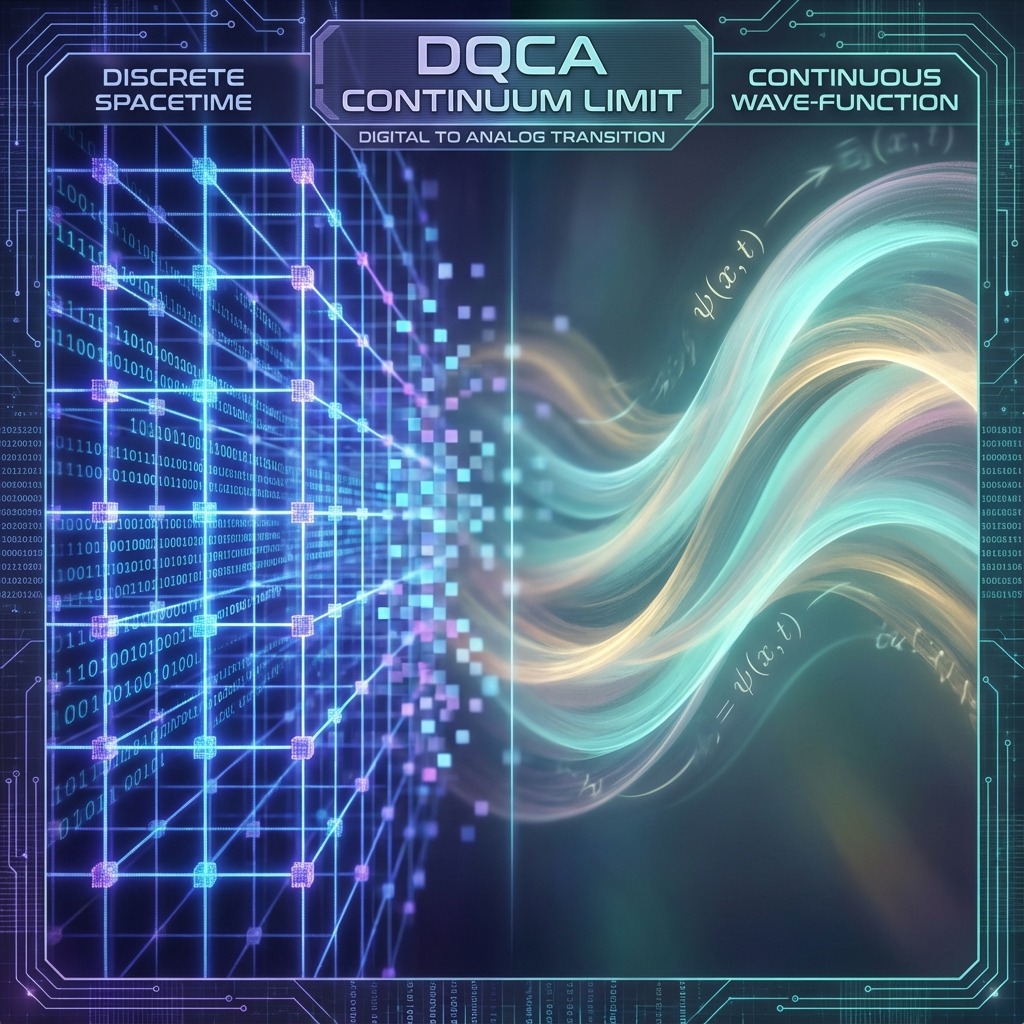
\includegraphics[width=0.8\textwidth]{images/appendix-b-dqca-continuum.png}
\caption{The emergence of the Dirac continuum from the underlying discrete automaton network.}
\label{fig:dqca_continuum}
\end{figure}

\subsection{Discrete Evolution Operator}
Consider a 1D lattice $\mathbb{Z}$ with state $\Psi(x,t) \in \mathbb{C}^2$. The unitary evolution $\hat{W}$ is:
\begin{equation}
    \hat{W} = \hat{S} \cdot \hat{C}, \quad \hat{S} = e^{-ik\sigma_z}, \quad \hat{C} = e^{i\theta \sigma_x}.
\end{equation}
In momentum space, this becomes:
\begin{equation}
    \tilde{W}(k) = \begin{pmatrix} e^{-ik} \cos\theta & i e^{-ik} \sin\theta \\ i e^{ik} \sin\theta & e^{ik} \cos\theta \end{pmatrix}.
\end{equation}

\subsection{Continuum Limit (\texorpdfstring{$\varepsilon \to 0$}{epsilon to 0})}
Let the lattice spacing be $\varepsilon$. We scale parameters as $k = p\varepsilon$, $\theta = m\varepsilon$, and $E_{phys} = \omega / \varepsilon$.
Expanding $\tilde{W}$ to first order in $\varepsilon$:
\begin{align}
    \tilde{W} &\approx \left( I - i p \varepsilon \sigma_z \right) \left( I + i m \varepsilon \sigma_x \right) \\
    &\approx I - i\varepsilon (p\sigma_z - m\sigma_x) + \mathcal{O}(\varepsilon^2).
\end{align}
Comparing this with the generator of time translation $e^{-i H_{eff} \varepsilon} \approx I - i H_{eff} \varepsilon$, we identify the effective Hamiltonian:
\begin{equation}
    H_{eff} = p\sigma_z - m\sigma_x.
\end{equation}
Solving for the eigenvalues $E$ of $H_{eff}$:
\begin{equation}
    \det(H_{eff} - E) = p^2 + m^2 - E^2 = 0 \implies E^2 = p^2 + m^2.
\end{equation}
This allows us to recover the relativistic dispersion relation from a strictly unitary discrete process.

\subsection{Lorentz Violation and Dispersion}
At order $\mathcal{O}(\varepsilon^2)$, the Baker-Campbell-Hausdorff formula gives a correction:
\begin{equation}
    H_{eff}^{(2)} = H_{Dirac} - \varepsilon p m \sigma_y.
\end{equation}
The exact dispersion relation derived from the trace of $\tilde{W}$ is:
\begin{equation}
    \cos(E\varepsilon) = \cos(p\varepsilon)\cos(m\varepsilon).
\end{equation}
For high-energy photons ($m=0$), the group velocity becomes energy-dependent:
\begin{equation}
    v_g(E) \approx 1 - \frac{1}{8} \left( \frac{E}{E_P} \right)^2.
\end{equation}
This prediction of a frequency-dependent speed of light for gamma rays is a key falsifiable signature of the theory (as discussed in Part VI).

\section{Dictionary: Omega Theory vs. Standard Physics}
\label{app:dictionary}

To facilitate translation between this axiomatic framework and standard contemporary physics, we provide the following dictionary:

\begin{table}[h]
\centering
\begin{tabular}{|l|l|}
\hline
\textbf{Standard Model / QFT / GR} & \textbf{Omega Theory (Digital Ontology)} \\ \hline
Spacetime Manifold & Dynamic Graph $\Lambda(t)$ (Quasicrystal) \\ \hline
Time $t$ & Global logic clock $\tau$ (Sequence Index) \\ \hline
Wavefunction $\Psi(x)$ & Local Qubit State $|\psi_x\rangle \in \mathbb{C}^d$ \\ \hline
Particle (Mass) & Topological Knot / Defect (Geometry) \\ \hline
Forces (Gauge Fields) & Curvature of Fiber Bundle ( Berry Core) \\ \hline
Gravity (Metric) & Entanglement Density / Information Flow \\ \hline
Speed of Light $c$ & Max Info Propagation Rate (Causality) \\ \hline
Planck Scale $l_P$ & Lattice Constant $\varepsilon$ (Pixel Size) \\ \hline
Vacuum Energy & Holographic Bond Saturation \\ \hline
Collapse of Wavefunction & Unitary Update by Observer Operator $\mathcal{C}$ \\ \hline
\end{tabular}
\caption{Conceptual mapping between continuous physics and discrete information theory.}
\end{table}

\section{Pseudocode: The Omega Evolution Algorithm}
\label{app:pseudocode}

The definitions in Part III can be operationalized as a computer simulation. The following pseudocode describes the fundamental loop of the universe:

\begin{verbatim}
# Global Constants
PHI = 1.6180339887... # Logic: Golden Ratio
PI  = 3.1415926535... # Geometry: Circle Constant
E   = 2.7182818284... # Dynamics: Growth Base

# Initialize Universe
Graph G = GeneratePenroseTiling(N_pixels)
State Vector |Omega> = Normalize(RandomComplexVector(G.size))

# MAIN TIME LOOP (The "Now")
for tau in 0 to INFINITY:
    
    # 1. Update Geometry (Metric Phase)
    #    Rotate phase of each node based on connectivity (Curvature)
    for node n in G:
        local_energy = Hamiltonian(n, G.neighbors(n))
        n.phase -= local_energy * delta_tau
        
    # 2. Update Topology (Matter/Forces)
    #    Check for knot stability; if unstable, decay
    knots = IdentifyTopologicalKnots(G)
    for k in knots:
        if k.winding_number > 1:
            Decay(k) # e.g., Muon -> Electron
            
    # 3. Holographic Constraint (Gravity)
    #    Enforce area law on causal horizons
    for region R in G:
        entropy = EntanglementEntropy(R)
        area    = BoundaryArea(R)
        if entropy > area / 4:
            ExpandSpace(R) # Dark Energy / Expansion
            
    # 4. Observer Measurement (Collapse/Choice)
    #    Self-referential check for complexity
    if Complexity(|Omega>) > Threshold:
        ApplyObserverOperator(|Omega>) # Downward Causation

    # 5. Advance Global Clock
    tau += 1
\end{verbatim}

\section{The Cosmic Trinity: \texorpdfstring{$\pi, e, \phi$}{pi, e, phi}}
\label{app:cosmic_trinity}

We conclude with a formal definition of the roles of the three fundamental dimensionless constants in Omega Theory.

\subsection{Physical Ontology}
We define the "Cosmic Trinity" of constants governing the three aspects of the computational universe:

\begin{figure}[ht]
\centering
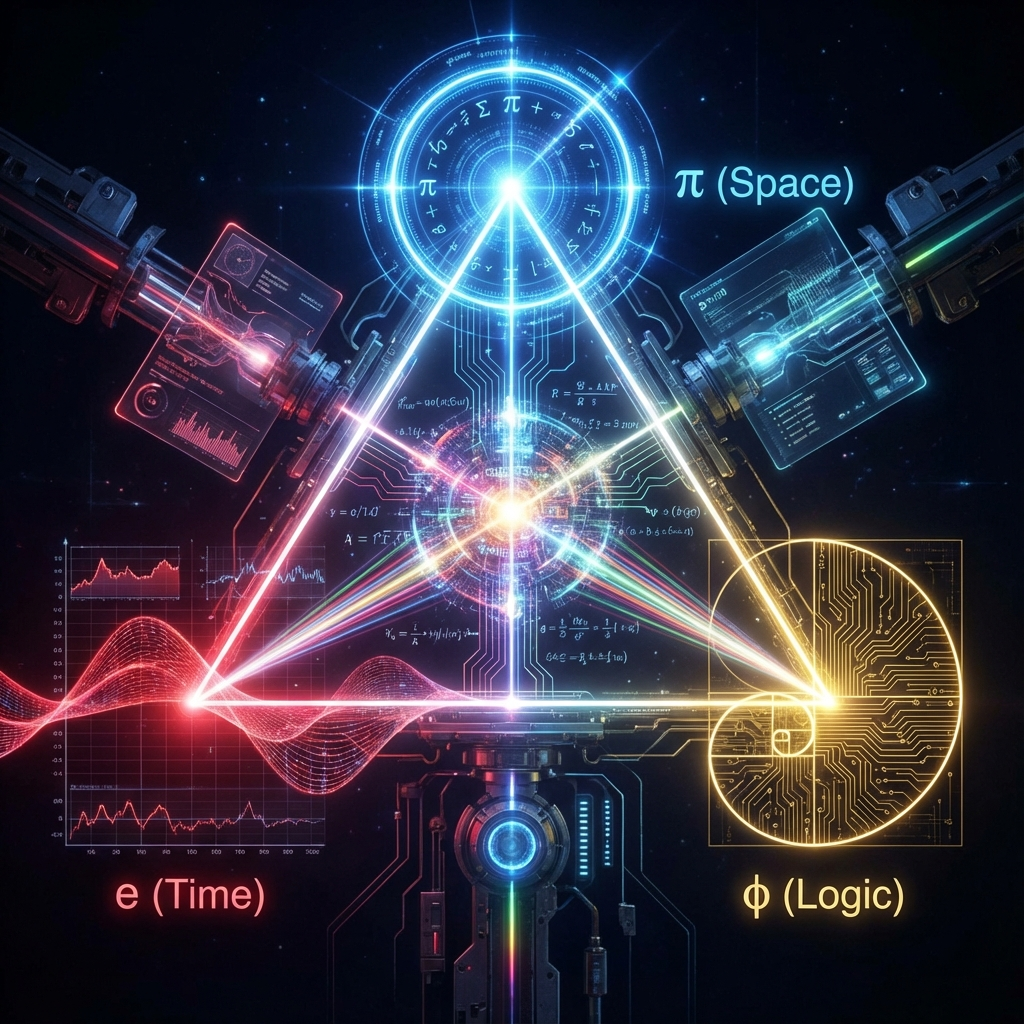
\includegraphics[width=0.8\textwidth]{images/appendix-f-cosmic-trinity.png}
\caption{The Cosmic Trinity: $\pi$, $e$, and $\phi$ as the foundational constants of geometry, dynamics, and logic.}
\label{fig:cosmic_trinity}
\end{figure}

\begin{enumerate}
    \item \textbf{$\pi$ (Space/Geometry)}: Defines the \textbf{Holographic Horizon}. It normalizes the total information capacity of the Hilbert space (volume of unit sphere) and imposes the Bekenstein bound.
    \item \textbf{$e$ (Time/Dynamics)}: Defines the \textbf{Unitary Evolution}. As the base of the time translation operator $U(t) = e^{-iHt}$, it ensures continuity and conservation of probability flow.
    \item \textbf{$\phi$ (Logic/Structure)}: Defines the \textbf{Discrete Encoding}. As the "most irrational" number, it ensures non-ergodic mixing (Chapter 17), preventing Poincaré recurrence and allowing the generation of infinite, non-repeating complexity (fractal structure).
\end{enumerate}

\subsection{Unified Operator Relation}
The generation of physical reality $\mathcal{R}$ can be symbolically expressed as the action of dynamics on geometry, modulated by logic:
\begin{equation}
    \mathcal{R} \sim \underbrace{e}_{\text{Dynamics}} \left( i \cdot \underbrace{2\pi}_{\text{Geometry}} \cdot \underbrace{\phi}_{\text{Logic}} \tau \right).
\end{equation}
This generalizes Euler's identity to a "Golden Identity" for an evolving universe, where the closed circle ($\pi$) is broken into an open spiral ($\phi$) driven by unitary flow ($e$).


\section*{Declarations}

\textbf{Ethics Approval and Consent to Participate}: Not applicable. This study does not involve human or animal subjects.

\textbf{Consent for Publication}: Not applicable.

\textbf{Availability of Data and Materials}: All data generated or analyzed during this study are included in this published article (and its supplementary information files). No external datasets were used.

\textbf{Competing Interests}: The author declares no competing interests. The affiliation with AELF PTE LTD. does not imply any commercial or financial conflict regarding the theoretical physics content of this work.

\textbf{Funding}: This research received no specific grant from any funding agency in the public, commercial, or not-for-profit sectors.

\textbf{Authors' Contributions}: HM is the sole author of this work.

\textbf{Acknowledgements}: The author thanks the collaborative AI assistant (Antigravity) for assistance with LaTeX typesetting and drafting.

\bibliographystyle{unsrt}
\bibliography{references}

\end{document}
